\documentclass[11pt,a4paper,openany]{report}
\usepackage[T1]{fontenc}
\usepackage[utf8]{inputenc}
\usepackage{lmodern}
\usepackage{microtype}
\usepackage{amsmath,amssymb,amsthm,mathtools,bm}
\usepackage{booktabs,array,longtable,tabularx}
\usepackage{xcolor}
\usepackage[margin=24mm,headheight=23pt]{geometry}
\usepackage{enumitem}
\usepackage{fancyhdr}
\usepackage{fancyvrb}
\usepackage{graphicx}
\usepackage{url}
\usepackage{xurl}
\usepackage{hyperref}

\definecolor{finblue}{HTML}{1F5A99}
\definecolor{fingreen}{HTML}{19733A}
\definecolor{finorange}{HTML}{D55E00}
\definecolor{finred}{HTML}{A61B1B}
\definecolor{finviolet}{HTML}{6A3D9A}

\hypersetup{
  unicode=true,
  colorlinks=true,
  linkcolor=finblue,
  citecolor=fingreen,
  urlcolor=finblue,
  pdftitle={FIN Programs 204--216: Categorical Measures, Perfect References, and External Falsification Gates},
  pdfauthor={Krzysztof Żuchowski},
  pdfsubject={Categorical state selection, exponent cocycles, symmetry-reference catalysis, finite-shot inference and external spectral falsification},
  pdfkeywords={FIN, spectral theory, Morita equivalence, operator algebra, catalytic asymmetry, Dirichlet form, conformal e-process, moment problem, operational physics}
}

\pagestyle{fancy}
\fancyhf{}
\fancyhead[L]{\small FIN Programs 204--216}
\fancyhead[R]{\small Release 10.19}
\fancyfoot[C]{\thepage}
\setlength{\parindent}{0pt}
\setlength{\parskip}{0.55em}
\setlist{nosep,leftmargin=2em}
\setcounter{tocdepth}{2}
\setcounter{secnumdepth}{3}
\emergencystretch=3em

\newcommand{\one}{\bm 1}
\newcommand{\C}{\mathbb C}
\newcommand{\R}{\mathbb R}
\newcommand{\Z}{\mathbb Z}

\begin{document}
\hypersetup{pageanchor=false}
\begin{titlepage}
\centering
\vspace*{8mm}
{\Large\bfseries FIN Research Monograph --- Release 10.19\par}
\vspace{10mm}
{\Huge\bfseries FIN Programs 204--216\par}
\vspace{6mm}
{\Large Categorical Measures, Perfect References,\\
and External Falsification Gates\par}
\vspace{16mm}
{\Large Krzysztof \.Zuchowski\par}
\vspace{2mm}
{\normalsize Independent Researcher --- Fractal Information Theory Project\par}
\vspace{2mm}
{\normalsize ORCID: \href{https://orcid.org/0009-0002-0909-3613}{0009-0002-0909-3613}\par}
\vspace{10mm}
{\large 27 July 2026\par}
{\normalsize Publication --- Preprint; record version 1.0.0\par}
\vfill
\begin{minipage}{0.88\textwidth}
\small
\textbf{Scope.} Thirteen executed studies of categorical central measures,
exponent cocycles, formal certification, catalytic symmetry references,
hidden mixing, sequential open-set detection, finite-shot process
tomography, environmental moment bounds, phase naturality, scale-free
spectral falsification, external intake, and prediction gating.

\medskip
\textbf{Central result.} Morita-permutation invariance conditionally selects
uniform central weights, while naturality under all unital homomorphisms is
impossible. A perfect asymmetric \(\mathbb Z_2\) reference enables exact
catalytic conversion but supplies, rather than derives, the missing
orientation bit.

\medskip
\textbf{Guardrail.} No QW-2191 discharge, strict selector, canonical physical
unit, target-independent strict exponent source, completed legacy--strict
bridge, role transfer, \(L_{\rm total}\), external physical validation, or
Theory-of-Everything closure is claimed.

\medskip
\textbf{License.} Creative Commons Attribution 4.0 International (CC BY 4.0).
\end{minipage}
\vfill
\end{titlepage}
\hypersetup{pageanchor=true}

\pagenumbering{roman}
\chapter*{Publication statement}
\addcontentsline{toc}{chapter}{Publication statement}
This release reports Programs 204--216 and recommends Programs 217--229.
Analytic proofs, exact finite computation, machine-checked proof fragments,
synthetic evidence, conditional constructions, unavailable infrastructure,
and failed external-data gates are kept separate.

\tableofcontents
\clearpage
\pagenumbering{arabic}

\section{Confidence convention}

The report distinguishes analytic proof, exact finite computation, machine-checked fragments, synthetic evidence, conditional construction, and open obligations. No unavailable certificate or external result is promoted by prose.

\chapter{Abstract}

This monograph reports thirteen executed research programs, numbered 204 through 216. They continue the study of the dimensionless FIN spectral core at the point where a self-adjoint operator already generates wave, heat, and Green dynamics, but a state, selector, physical scale, apparatus, and independent empirical record are not generated by the spectral theorem.

The first result sharpens the central-state problem. If the simple summands of a finite semisimple algebra are required to be interchangeable under a Morita-permutation principle, the unique normalized central measure is uniform. For the FIN dimension vector \((1,2,2,2,2)\) this gives the exact expectation \(9/5\). The normalized represented-space trace instead gives \(17/9\) and violates the added permutation principle. This is conditional uniqueness, not a strict FIN derivation. Moreover, no automorphism-natural state assignment can be contravariantly natural under all unital \(*\)-homomorphisms: the map

\[
f:\mathbb C^2\longrightarrow\mathbb C^3,
\qquad
f(a,b)=(a,b,b)
\]

pulls the uniform state on \(\mathbb C^3\) back to \((1/3,2/3)\), whereas automorphism naturality on \(\mathbb C^2\) demands \((1/2,1/2)\).

The second result classifies continuous one-parameter exponent cocycles. Every continuous solution of

\[
b(t+s)=b(t)+b(s)
\]

is \(b(t)=\kappa t\). Moving the legacy exponent \(1\) to the strict exponent \(9/5\) therefore fixes only \(\kappa t_*=4/5\), not either factor. Multiplicative and fixed-point flows have the same nonselection defect. The strict exponent cannot be recovered from semigroup form alone.

The third principal result concerns symmetry resources. A catalyst invariant under the reflection cannot repair a violated one-copy Alberti--Uhlmann inequality. In contrast, the perfectly asymmetric reference

\[
\Pi_+=\frac{I+\sigma_x}{2}
\]

supports an explicit covariant measure-and-prepare channel that maps the declared source to any prescribed target while returning \(\Pi_+\) exactly. The construction is a valid operational completion, but it supplies a perfect orientation bit. It neither derives that bit from the strict kernel nor discharges the strict-core selector obstruction QW-2191.

The round also supplies a hidden-mixing confidence theorem using Berbee coupling and thinning; a time-uniform conformal e-process with exact null control under fresh calibration; conservative finite-shot process-tomography regions; and a sharp trigonometric moment interval. Given a real symmetric environmental phase law with first moment \(c_1=4/5\), positivity of

\[
T_2=
\begin{pmatrix}
1&c_1&c_2\\
c_1&1&c_1\\
c_2&c_1&1
\end{pmatrix}
\]

gives the exact and attainable interval

\[
\frac{7}{25}\le c_2\le 1.
\]

A phase-source hierarchy extends the naturality obstruction from continuous circle homomorphisms to Borel homomorphisms and trivial-action continuous one-cocycles. None maps the order-eight legacy phase to the non-torsion strict phase without target-coded data.

Finally, a scale-free spectral fingerprint is preregistered and challenged. It is invariant over twelve decades of operator scaling and under node relabeling, accepts a one-percent edge perturbation, and rejects a ten-percent perturbation, the nearest-neighbour cycle, and the raw legacy generator. This is an internally falsifiable operator protocol, not experimental physics. A fresh audit finds no independent external record satisfying the frozen eleven-field intake gate. The external prediction remains locked.

The proof infrastructure is reported without concealment. A dependency-free Lean 4 core probe compiles in the local toolchain and 200 exact rational Dirichlet witnesses pass. The proposed general graph library does not compile because Mathlib is not installed in the clean environment. Arb and python-flint remain unavailable, and Docker server access is denied. No formal sub-three-percent fractional certificate is claimed.

No non-premise strict selector, canonical physical unit, target-independent strict exponent or compression source, completed legacy-to-strict bridge, legacy role transfer, role-bearing \(L_{\rm total}\), external physical validation, or Theory-of-Everything closure is asserted.

\par\medskip\hrule\medskip

\chapter{Executive summary}

\section{Outcome table}

\begin{center}
\begingroup\small
\setlength{\tabcolsep}{3.5pt}
\renewcommand{\arraystretch}{1.16}
\begin{longtable}{@{}p{0.071\textwidth}p{0.377\textwidth}p{0.226\textwidth}p{0.186\textwidth}@{}}
\toprule
\textbf{Program} & \textbf{Constructed object} & \textbf{Main result} & \textbf{Confidence} \\
\midrule
\endhead
204 & MoritaCentralTrace & uniform central weights are unique under an added Morita-permutation axiom; all-homomorphism naturality is impossible & Proven, conditional premise \\
205 & ExponentCocycleModuli & continuous flow form does not select \(9/5\) & Proven in class \\
206 & CertificationEnvironmentContract & reproducible Arb contract frozen; engine unavailable & Proven audit \\
207 & FormalBuildContract & Lean core probe compiles; general Mathlib library remains open & Machine-checked core; general proof open \\
208 & PerfectZ2ReferenceCatalyst & invariant catalysts do not help; a perfect asymmetric bit enables exact conversion & Proven \\
209 & CoupledThinningFrame & valid hidden-mixing bound under calibrated geometric mixing & Proven conditionally \\
210 & IndependentBlockConformalEProcess & exact time-uniform null test with strong synthetic power & Proven null law; strong evidence \\
211 & FiniteShotProcessRegion & simultaneous finite-shot region and memory test & Proven construction; strong evidence \\
212 & ToeplitzMomentInterval & sharp \(c_2\in[7/25,1]\) & Proven \\
213 & PhaseNaturalityHierarchyCertificate & phase no-go extends through measurable homomorphisms & Proven in declared hierarchy \\
214 & ProjectiveSpectralFingerprintProtocol & scale-free operator fingerprint frozen and challenged & Proven invariance; finite computation \\
215 & IndependentExternalBundleRequest & no local candidate passes the independent 11/\allowbreak{}11 gate & Proven local audit \\
216 & ConditionalPredictionLock & external prediction correctly not executed & Proven gate status \\
\bottomrule
\end{longtable}
\endgroup
\end{center}

\section{Central conclusion}

The round identifies three mathematically different kinds of missing data.

First, \textbf{categorical section data} are needed when the spectral algebra has nontrivial centre. A state on each matrix block does not determine the weights between blocks.

Second, \textbf{asymmetry resources} are needed when an operation must choose a direction in a reflection orbit. The perfect reference construction proves that such a resource is sufficient. The invariant-catalyst theorem proves that symmetry-preserving ancillary data are insufficient.

Third, \textbf{operational and empirical data} are needed to turn a projective spectral signature into a physical claim. The operator determines an internally testable dimensionless fingerprint; it does not determine which apparatus reconstructs it or provide an independent measurement record.

The minimal operational extension visible after Programs 204--216 is therefore not a new kernel. It is a typed package

\[
\mathfrak E=
(\mathcal A,\rho,\Gamma,A,\mathcal I,\mathcal C,\mathcal M,\mathcal R),
\]

where \(\mathcal A\) is an observable algebra, \(\rho\) a state, \(\Gamma\) a symmetry action, \(A\) the spectral generator, \(\mathcal I\) an intervention family, \(\mathcal C\) a clock and scale calibration, \(\mathcal M\) a measurement instrument, and \(\mathcal R\) an independently sourced ordered record. Programs 204, 208, and 214--216 show respectively why \(\rho\), an orientation resource inside \(\mathcal I\), and \(\mathcal R\) cannot be silently recovered from \(A\).

\section{Strongest new theorem}

The most conceptually decisive result is the perfect-reference dichotomy. Let \(\Theta(\rho)=R\rho R\) be the \(\mathbb Z_2\) reflection. If a catalyst \(\kappa\) is invariant, then for every \(q\ge0\),

\[
\left\|
\rho\otimes\kappa-q\,\Theta(\rho)\otimes\kappa
\right\|_1
=
\left\|\rho-q\,\Theta(\rho)\right\|_1.
\]

Any violated trace-norm conversion inequality remains violated. Symmetric catalysis cannot manufacture a selector.

For \(\Pi_\pm=(I\pm\sigma_x)/2\), define

\[
\mathcal E(X)=
\operatorname{tr}[(I\otimes\Pi_+)X]\,\tau\otimes\Pi_+
+
\operatorname{tr}[(I\otimes\Pi_-)X]\,\Theta(\tau)\otimes\Pi_-.
\]

This channel is completely positive, trace preserving, and covariant under \(R\otimes R\). For every source \(\rho\),

\[
\mathcal E(\rho\otimes\Pi_+)=\tau\otimes\Pi_+.
\]

Thus a perfect reference is sufficient and exactly reusable. It is not free: its two group-orbit states are orthogonal, so it contains a full classical orientation bit. The selector problem has been converted into a resource provenance problem rather than solved by the strict kernel.

\section{What remains blocked}

\begin{itemize}
\item 
Morita-permutation invariance is not sourced as a preparation law.

\item 
No flow principle selects the exponent increment \(4/5\).

\item 
The full Arb certificate has not run.

\item 
The Mathlib-dependent Lean library has not compiled.

\item 
No strict source supplies the perfect reference orientation.

\item 
The hidden-mixing theorem still needs a calibrated lower refresh bound.

\item 
No strict phase source survives the naturality hierarchy.

\item 
No canonical dimensional unit is exported.

\item 
No external bundle satisfies all eleven frozen fields.

\item 
External prediction and physical validation remain unexecuted.

\end{itemize}

\par\medskip\hrule\medskip

\chapter{Scope and mathematical core}

\section{Kernel split}

The legacy and strict kernels are kept separate:

\[
K_{\rm legacy}(d)=
\alpha_{\rm geo}
\frac{\cos(\omega_\ell d+\phi_\ell)}
{1+\beta_{\rm tors}d},
\]

where

\[
\omega_\ell=\frac{\pi}{4},
\quad
\phi_\ell=\frac{\pi}{6},
\quad
\beta_{\rm tors}=0.01,
\quad
\alpha_{\rm geo}=4\ln2,
\]

and

\[
K_{\rm strict}(d)=
\frac{\cos(\omega_s d+\phi_s)}
{1+\beta_s d^{\eta_s}},
\]

where

\[
\omega_s=0.18575,
\quad
\phi_s=0.16250,
\quad
\beta_s=1,
\quad
\eta_s=\frac95.
\]

The legacy kernel remains an intermediate bridge kernel. The strict kernel is the later enriched working kernel. Programs 205 and 213 ask whether exponent and phase could arise from natural transformation laws. Their negative answers do not demote either kernel, identify the kernels, or authorize transfer of legacy physical roles.

\section{Spectral engine}

On a finite vertex set, let \(W=W^*\) be a nonnegative symmetric weight matrix with constant row sum \(s\). Define

\[
A=sI-W.
\]

Then

\[
\langle f,Af\rangle
=
\frac12\sum_{x,y}W_{xy}|f_x-f_y|^2\ge0.
\]

Consequently one operator generates

\[
U_t=e^{-itA},
\qquad
P_t=e^{-tA},
\qquad
G_z=(A+zI)^{-1}.
\]

Here \(U_t\) is unitary wave evolution, \(P_t\) is a positivity-preserving stochastic heat semigroup, and \(G_z\) is a screened Green operator for \(z>0\). This common origin is theorem-level finite operator theory. It does not choose a state, an arrow of time, a dimensional clock, or a measurement record.

For the twelve-node strict circulant used in Program 214,

\[
s=1.6603072787660986,
\]

numerically consistent with the previously recorded value \(1.660307278766099\).

\section{Confidence convention}

The report uses four levels.

\begin{itemize}
\item 
\textbf{Proven:} an analytic proof or an exact finite derivation is supplied.

\item 
\textbf{Proven, computer-assisted:} the claim is finite and covered by executable checks with frozen inputs.

\item 
\textbf{Strong evidence:} repeated numerical experiments support a clearly scoped proposition but do not replace a proof.

\item 
\textbf{Open or conditional:} a premise, toolchain, external record, or theorem remains absent.

\end{itemize}

Synthetic data validate methods only. Local provenance audits validate only the local workspace. A contract is not a certificate, and a preregistration is not a successful experiment.

\section{Reproducible methodology}

All Programs 204--216 are generated by one deterministic Python suite with seed 20260727. The release contains machine-readable results, one figure per program, immutable protocol contracts, two Lean sources, and 77 regression and scientific-boundary tests. Those tests check not only numerical values but also negative claims: no selector, unit, bridge, role transfer, \(L_{\rm total}\), external validation, or Theory-of-Everything conclusion may appear in the result object.

\par\medskip\hrule\medskip

\chapter{Program 204 --- Morita-compatible central measures}

\section{Question}

For

\[
\mathcal A=\bigoplus_{i=1}^mM_{d_i}(\mathbb C),
\]

inner-unitary invariance forces a state to have the form

\[
\rho(a_1,\ldots,a_m)
=
\sum_{i=1}^m p_i\frac{\operatorname{Tr}(a_i)}{d_i},
\qquad
p_i\ge0,
\quad
\sum_i p_i=1.
\]

Can a categorical principle remove the central simplex \((p_i)\)?

\section{Conditional uniqueness theorem}

Assume in addition that all simple summands are interchangeable under a declared Morita-permutation action and that the state is invariant under this action. Every transposition gives \(p_i=p_j\). Therefore

\[
p_i=\frac1m.
\]

For \((d_i)=(1,2,2,2,2)\), the selected block-dimension expectation is

\[
\sum_i p_id_i
=
\frac{1+2+2+2+2}{5}
=
\frac95.
\]

The finite constraint matrix has rank \(4\) and nullity \(1\), confirming uniqueness after normalization.

The represented-space normalized trace instead uses

\[
p_i=\frac{d_i}{\sum_jd_j}
\]

and yields

\[
\sum_i p_id_i
=
\frac{1+4+4+4+4}{9}
=
\frac{17}{9}.
\]

Its maximum residual under permutations of the five central labels is \(1/9\).

\section{Global naturality no-go}

The preceding result depends on the chosen morphism class. There is no state assignment that is simultaneously automorphism-natural on every \(\mathbb C^n\) and contravariantly natural under every unital \(*\)-homomorphism.

Automorphism naturality makes the state on \(\mathbb C^2\) uniform. It also makes the state on \(\mathbb C^3\) uniform. For

\[
f(a,b)=(a,b,b),
\]

the pullback of the latter has weights \((1/3,2/3)\), contradicting \((1/2,1/2)\). The exact defect is \(1/6\).

\section{Falsification and verdict}

The value \(9/5\) is not derived merely by saying "Morita invariance." Morita equivalence preserves representation categories, not a canonical normalization of states. The report therefore exposes the required permutation-invariance axiom explicitly.

\textbf{Verdict --- Proven, conditional.} The added axiom is sufficient and uniquely selects \(9/5\). Current strict FIN does not supply it as a physical preparation rule.

\begin{figure}[htbp]
\centering
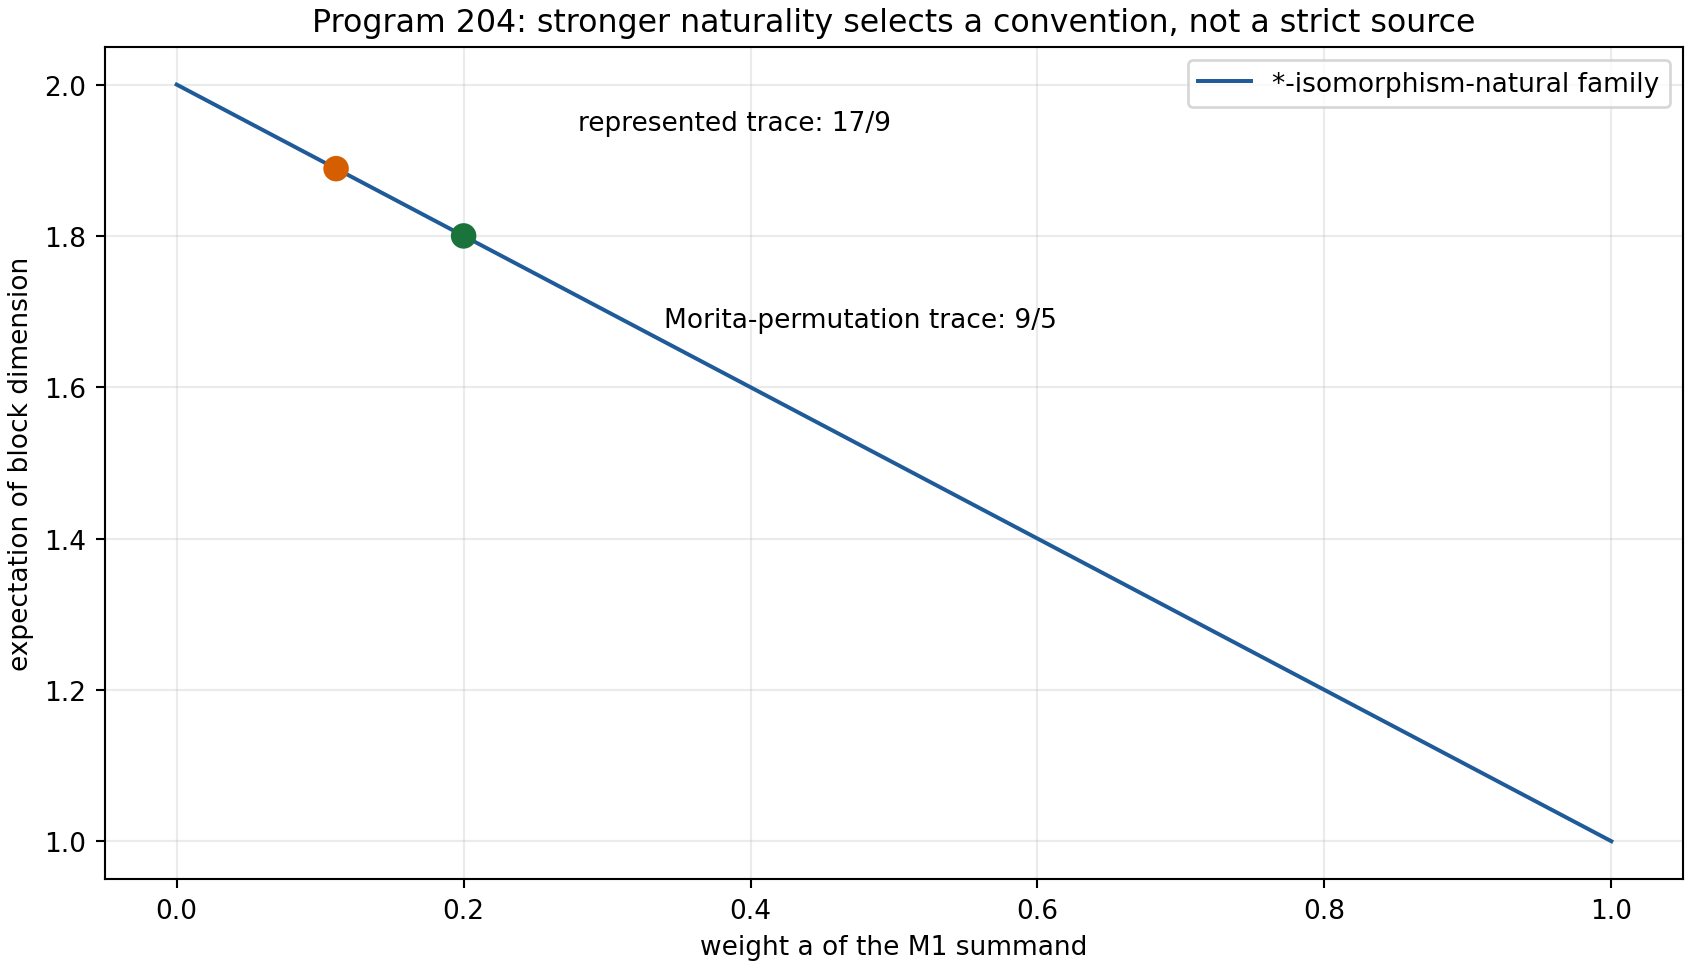
\includegraphics[width=0.94\textwidth]{FIN_Programs_204_216_Categorical_Catalytic_External_Figures/program204_morita_central_measure.png}
\caption{Morita-permutation invariance conditionally selects uniform central weights; the represented-space trace remains a different choice.}
\end{figure}

\par\medskip\hrule\medskip

\chapter{\texorpdfstring{Program 205 --- Exponent cocycles and the nonselection of \(9/5\)}{Program 205 --- Exponent cocycles and the nonselection of 9/\allowbreak{}5}}

\section{Additive cocycle theorem}

Suppose completion acts on the denominator exponent through

\[
\eta(t)=\eta_0+b(t)
\]

and composition requires

\[
b(t+s)=b(t)+b(s).
\]

Continuity gives the Cauchy-equation classification

\[
b(t)=\kappa t.
\]

Starting from \(\eta_0=1\) and reaching \(\eta_*=9/5\) requires

\[
\kappa t_*=\frac45.
\]

The suite displays 601 distinct rate-time pairs satisfying this equation. The maximum numerical cocycle residual is \(4.44\times10^{-16}\).

\section{Alternative flow families}

Three natural alternatives were tested.

\begin{enumerate}
\item 
A multiplicative flow \(\eta(t)=\eta_0e^{\kappa t}\) fixes only \(\kappa t_*=\log(9/5)\).

\item 
A stable fixed-point flow selects \(9/5\) only by inserting it as the fixed point parameter.

\item 
Multiplication by a monomial \(d^{b}\) changes the exponent by \(b\), but the required \(b=4/5\) remains unsourced.

\end{enumerate}

None turns semigroup form into a value-selection theorem.

\section{Separation from the beta gauge}

Under the positive length-scale action used previously,

\[
x=\beta^{1/\eta}d,
\qquad
\nu=\frac{\omega}{\beta^{1/\eta}},
\]

\(\eta\) is invariant. An exponent flow is therefore a new typed dynamical layer, not a reparametrization of \(\beta\).

\textbf{Verdict --- Proven in the continuous one-parameter class.} The flow law provides an interpolation family but not a target-independent source for \(9/5\).

\begin{figure}[htbp]
\centering
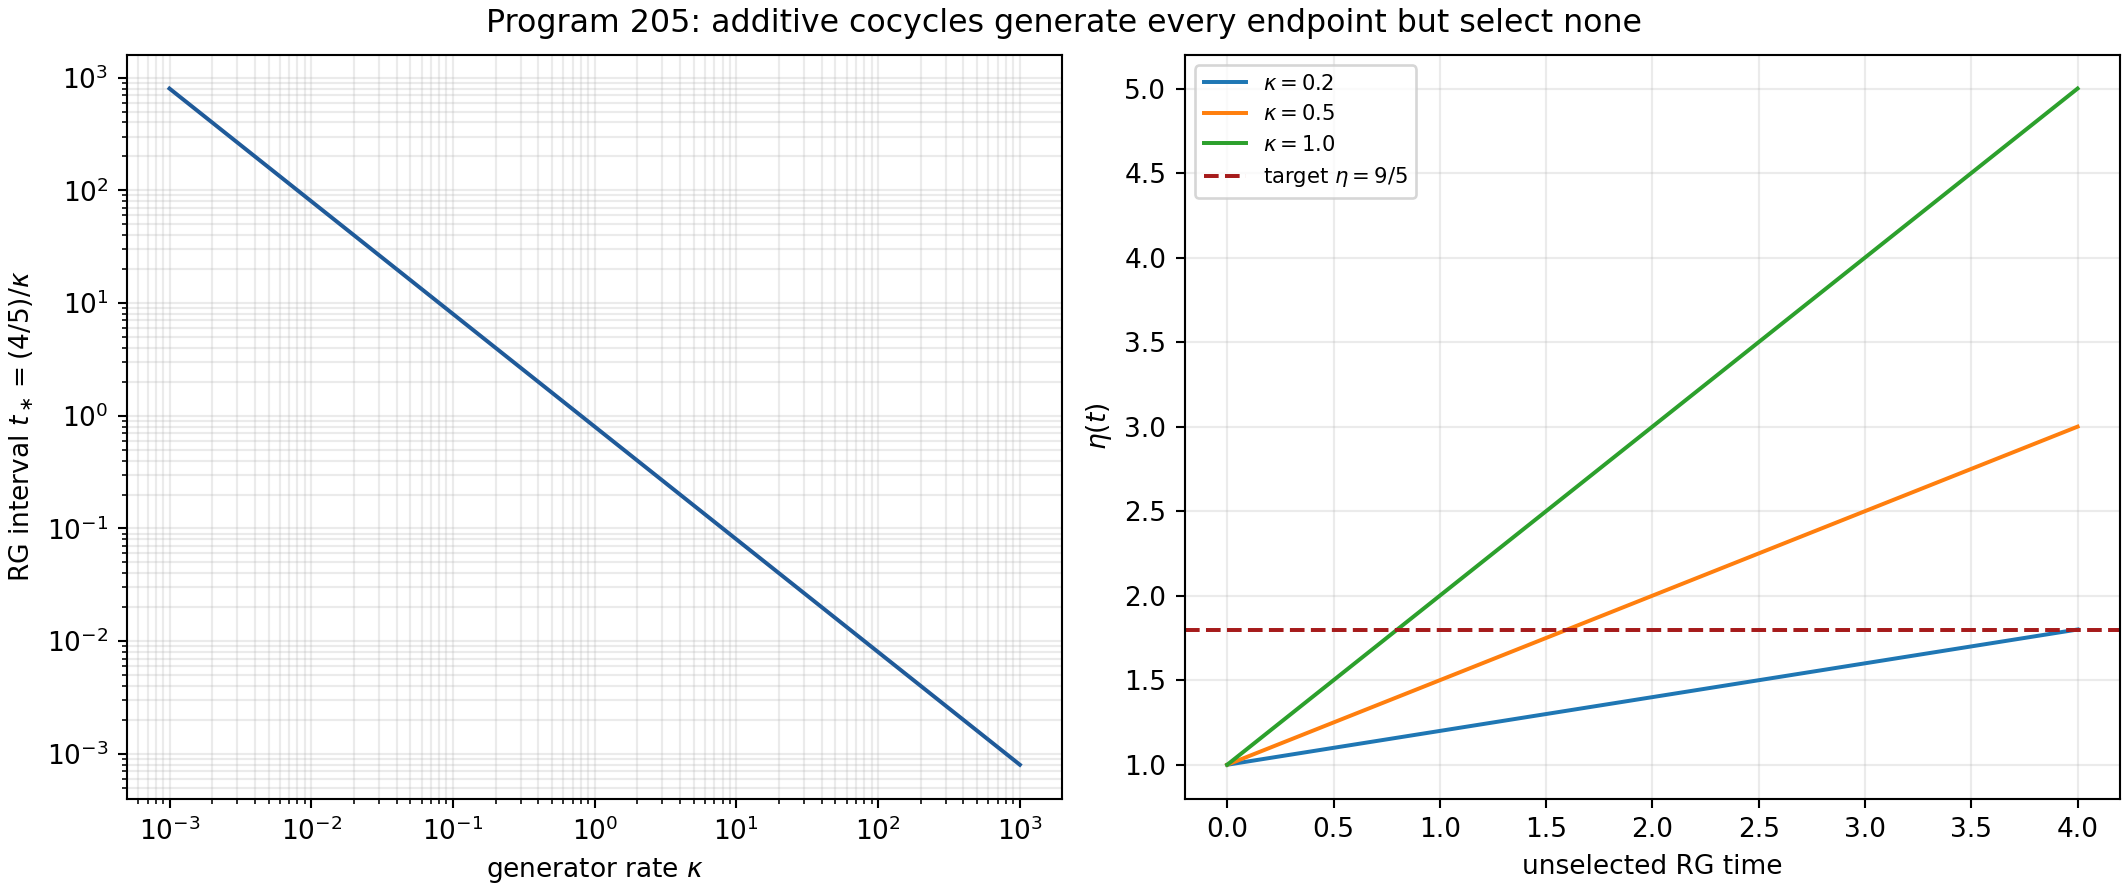
\includegraphics[width=0.94\textwidth]{FIN_Programs_204_216_Categorical_Catalytic_External_Figures/program205_eta_cocycle.png}
\caption{The additive exponent cocycle reaches \(9/5\) along infinitely many rate--time pairs and therefore does not select the endpoint.}
\end{figure}

\par\medskip\hrule\medskip

\chapter{Program 206 --- Arb certification environment}

The missing common directed-rounding computation was converted into a frozen CertificationEnvironmentContract. The contract records required package versions, hashes, entry points, rounding mode, input schema, and acceptance criterion.

The local audit found:

\begin{itemize}
\item 
python-flint: absent;

\item 
an arb executable: absent;

\item 
Docker command-line client: present;

\item 
Docker server: inaccessible because the socket denies permission;

\item 
inherited worst enclosure: \(0.6129831478193526\);

\item 
required threshold: \(0.03\);

\item 
formal five-node run: not executed.

\end{itemize}

These observations distinguish three statements that are often conflated:

\begin{enumerate}
\item 
a mathematical certificate specification exists;

\item 
a compatible implementation exists;

\item 
the certificate has been run and passed.

\end{enumerate}

Only the first is established here.

\textbf{Verdict --- Proven environment audit; certificate open.} No sub-three-percent formal enclosure is claimed.

\begin{figure}[htbp]
\centering
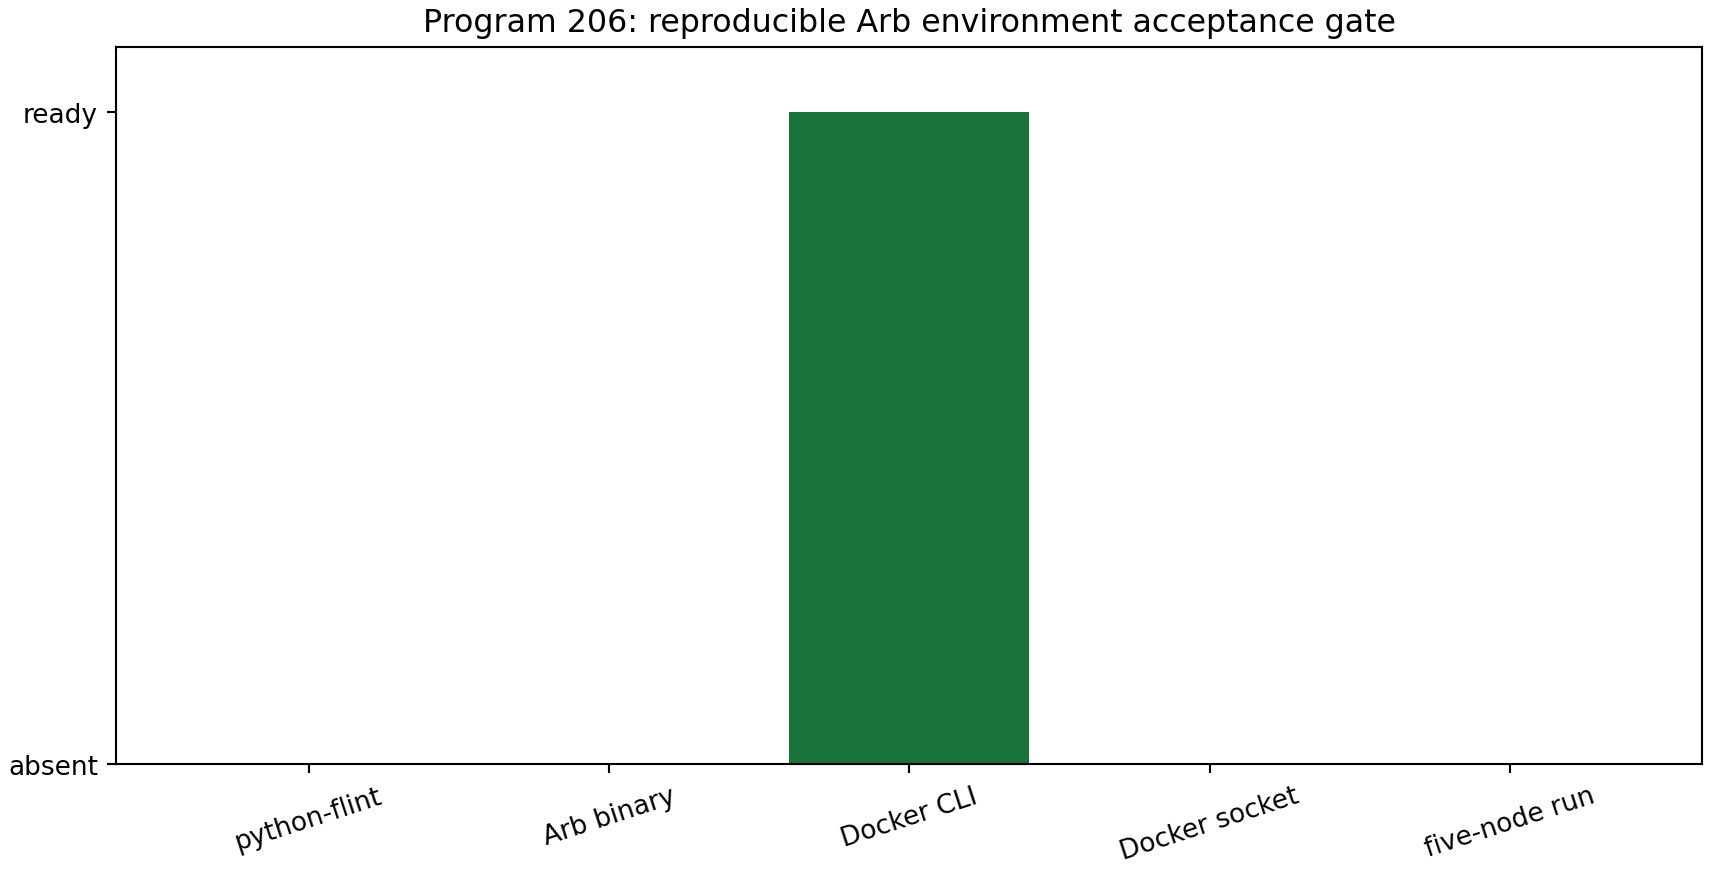
\includegraphics[width=0.94\textwidth]{FIN_Programs_204_216_Categorical_Catalytic_External_Figures/program206_arb_environment.png}
\caption{The reproducibility contract is complete, but the local Arb engine and Docker server are unavailable.}
\end{figure}

\par\medskip\hrule\medskip

\chapter{Program 207 --- Lean build closure}

\section{Two proof layers}

The study separates a dependency-free core from a general graph library. The local Lean 4.28.0 compiler machine-checks the core probe. Its exact evaluation returns 27, and its proposition is discharged by decide.

The general source states the intended finite weighted-graph objects:

\begin{itemize}
\item 
the Dirichlet quadratic identity;

\item 
positive semidefiniteness;

\item 
the constant vector in the kernel;

\item 
unitarity of \(e^{-itA}\);

\item 
entrywise nonnegativity and stochasticity of \(e^{-tA}\).

\end{itemize}

In a clean environment it fails immediately because the Mathlib module is not present. This is a dependency failure before theorem verification, not evidence that the theorems are false.

\section{Exact witness pack}

Independently of Lean, 200 new rational weighted-circulant cases were checked exactly. In every case,

\[
f^\mathsf TAf
=
\frac12\sum_{x,y}W_{xy}(f_x-f_y)^2
\ge0.
\]

Exact rational arithmetic eliminates floating-point ambiguity for these witnesses.

\section{Verdict}

\textbf{Machine-checked:} dependency-free core probe.\\
\textbf{Exactly checked:} 200 finite rational witnesses.\\
\textbf{Open:} general Mathlib-based library.

The report does not call the entire Dirichlet library formally verified.

\begin{figure}[htbp]
\centering
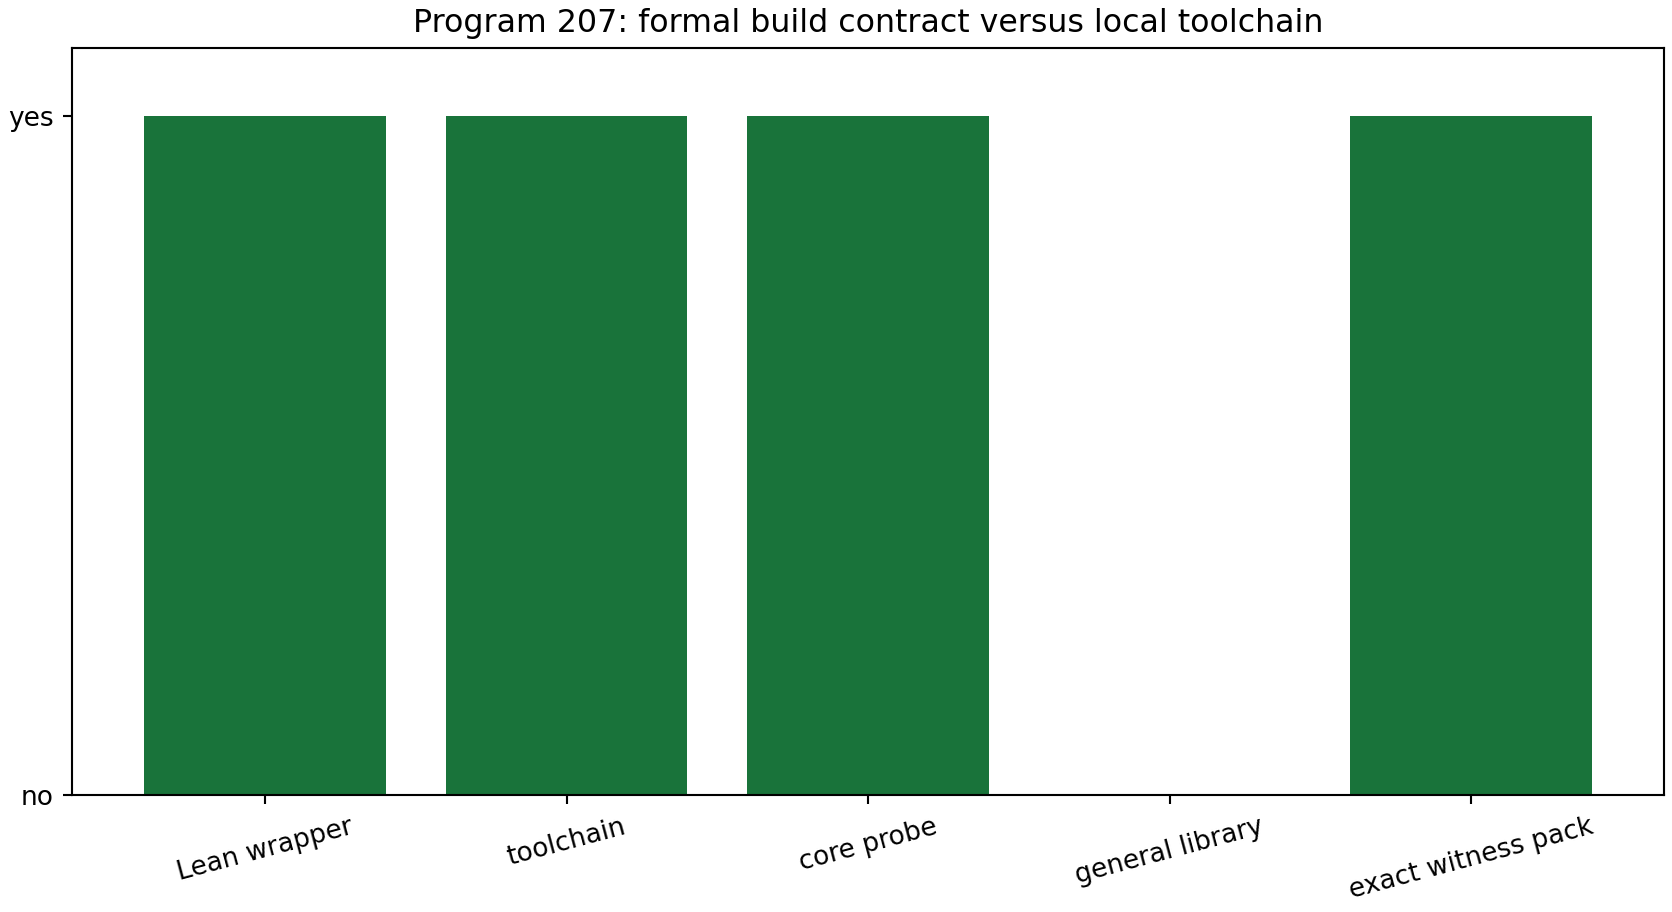
\includegraphics[width=0.94\textwidth]{FIN_Programs_204_216_Categorical_Catalytic_External_Figures/program207_lean_build.png}
\caption{The dependency-free Lean core compiles and the exact witness pack passes; the general Mathlib library remains uncompiled.}
\end{figure}

\par\medskip\hrule\medskip

\chapter{Program 208 --- Catalytic symmetry breaking}

\section{Invariant-catalyst no-help theorem}

Let \(\Theta(\rho)=R\rho R\) and suppose \(\Theta(\kappa)=\kappa\). If deterministic covariant conversion is tested by the family of trace-norm inequalities, tensoring both source and target with \(\kappa\) changes neither side:

\[
\|(\rho-q\Theta\rho)\otimes\kappa\|_1
=
\|\rho-q\Theta\rho\|_1\|\kappa\|_1
=
\|\rho-q\Theta\rho\|_1.
\]

Therefore an invariant catalyst cannot repair any violated member of the family.

\section{Perfect-reference construction}

Let reflection be conjugation by \(\sigma_z\) and let

\[
\Pi_\pm=\frac{I\pm\sigma_x}{2}.
\]

Reflection exchanges \(\Pi_+\) and \(\Pi_-\). For any target \(\tau\), the channel

\[
\mathcal E(X)=
\operatorname{tr}[(I\otimes\Pi_+)X]\,\tau\otimes\Pi_+
+
\operatorname{tr}[(I\otimes\Pi_-)X]\,\Theta(\tau)\otimes\Pi_-
\]

is a covariant measure-and-prepare channel. The finite Choi-equivalent tests give zero trace-preservation, covariance, and mapping residuals.

For the previously impossible conversion from Bloch coordinates \((0.6,0)\) to \((0.6,0.8)\),

\[
\mathcal E(\rho_{\rm source}\otimes\Pi_+)
=
\rho_{\rm target}\otimes\Pi_+.
\]

The target can be arbitrary.

\section{Imperfect references}

A scan of 100 imperfect transverse catalyst radii \(r_c<1\) leaves the best necessary trace-norm margin at

\[
-0.808036981970047.
\]

At \(r_c=1\), the margin reaches numerical zero \(-1.82\times10^{-12}\), consistent with the explicit channel. This scan is a necessary-condition falsification, not a full classification of approximate catalysis.

\section{Interpretation}

The perfect reference is not a hidden derivation of orientation. Its orbit states are orthogonal and can be measured without error. It supplies the missing orientation bit as an operational resource. This precisely explains why the construction succeeds and why it does not solve QW-2191.

\textbf{Verdict --- Proven.} Symmetric catalysts are useless in the declared test; a perfect asymmetric reference is sufficient but externally supplied.

\begin{figure}[htbp]
\centering
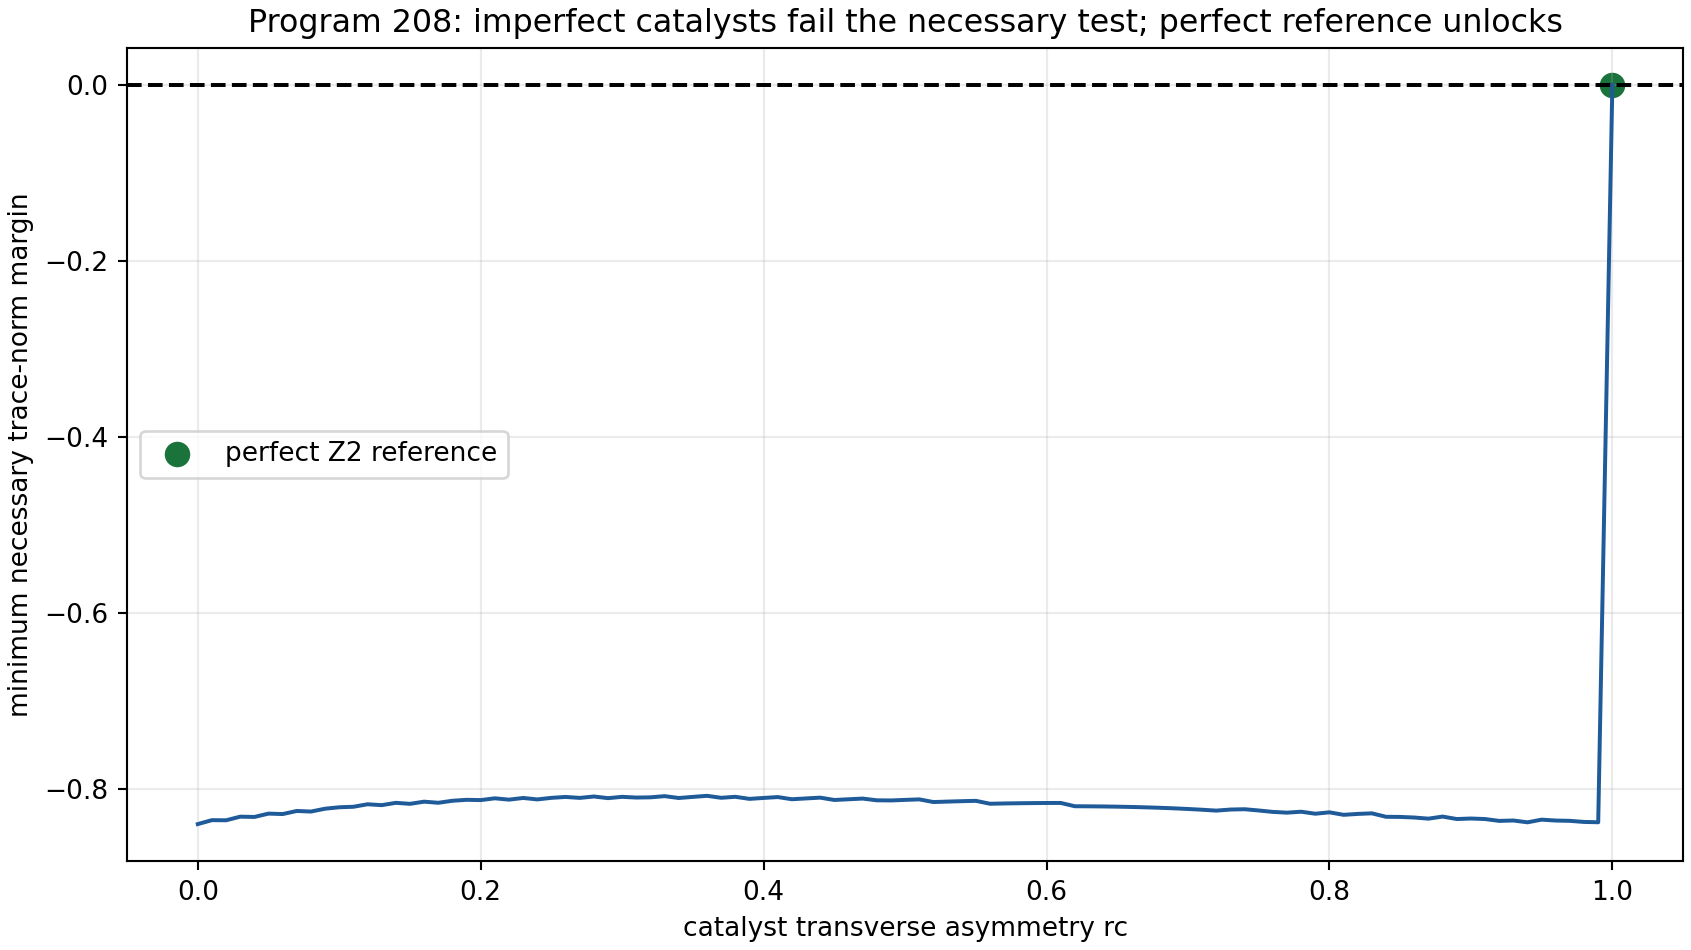
\includegraphics[width=0.94\textwidth]{FIN_Programs_204_216_Categorical_Catalytic_External_Figures/program208_catalytic_conversion.png}
\caption{Imperfect reference states fail the sampled necessary conversion test, whereas the perfect \(\mathbb Z_2\) reference reaches the exact boundary.}
\end{figure}

\par\medskip\hrule\medskip

\chapter{Program 209 --- Hidden mixing with calibrated coupling}

\section{Theorem}

Assume an unobserved-refresh process satisfies the certified bound

\[
\beta(k)\le(1-p_0)^k
\]

for known \(p_0>0\). Thin the record at lag \(L\), leaving \(m\) observations. Berbee coupling and the Dvoretzky--Kiefer--Wolfowitz inequality give

\[
\Pr(D_m>\varepsilon)
\le
2e^{-2m\varepsilon^2}
+
(m-1)\beta(L).
\]

This removes the need to observe the refresh flags. It does not remove the need to calibrate a mixing-rate lower bound.

\section{Challenge}

For \(n=10000\), calibrated \(p_0=0.05\), and true refresh probability \(0.06\), the rule selects

\[
L=166,
\qquad
m=61,
\qquad
(m-1)(1-p_0)^L=0.0120301.
\]

Across 240 stable-law simulations, treating all 10000 entries as independent gives coverage \(0.845833\). The coupling-valid construction gives coverage \(1.0\), but its mean exponent-interval width is \(6.58742\), compared with \(0.330159\) for the invalid nominal method.

The result is deliberately uncomfortable: rigor is recovered by paying a large information cost. The theorem prevents false precision rather than manufacturing power.

\textbf{Verdict --- Proven under the calibrated mixing envelope; strong numerical coverage evidence.}

\begin{figure}[htbp]
\centering
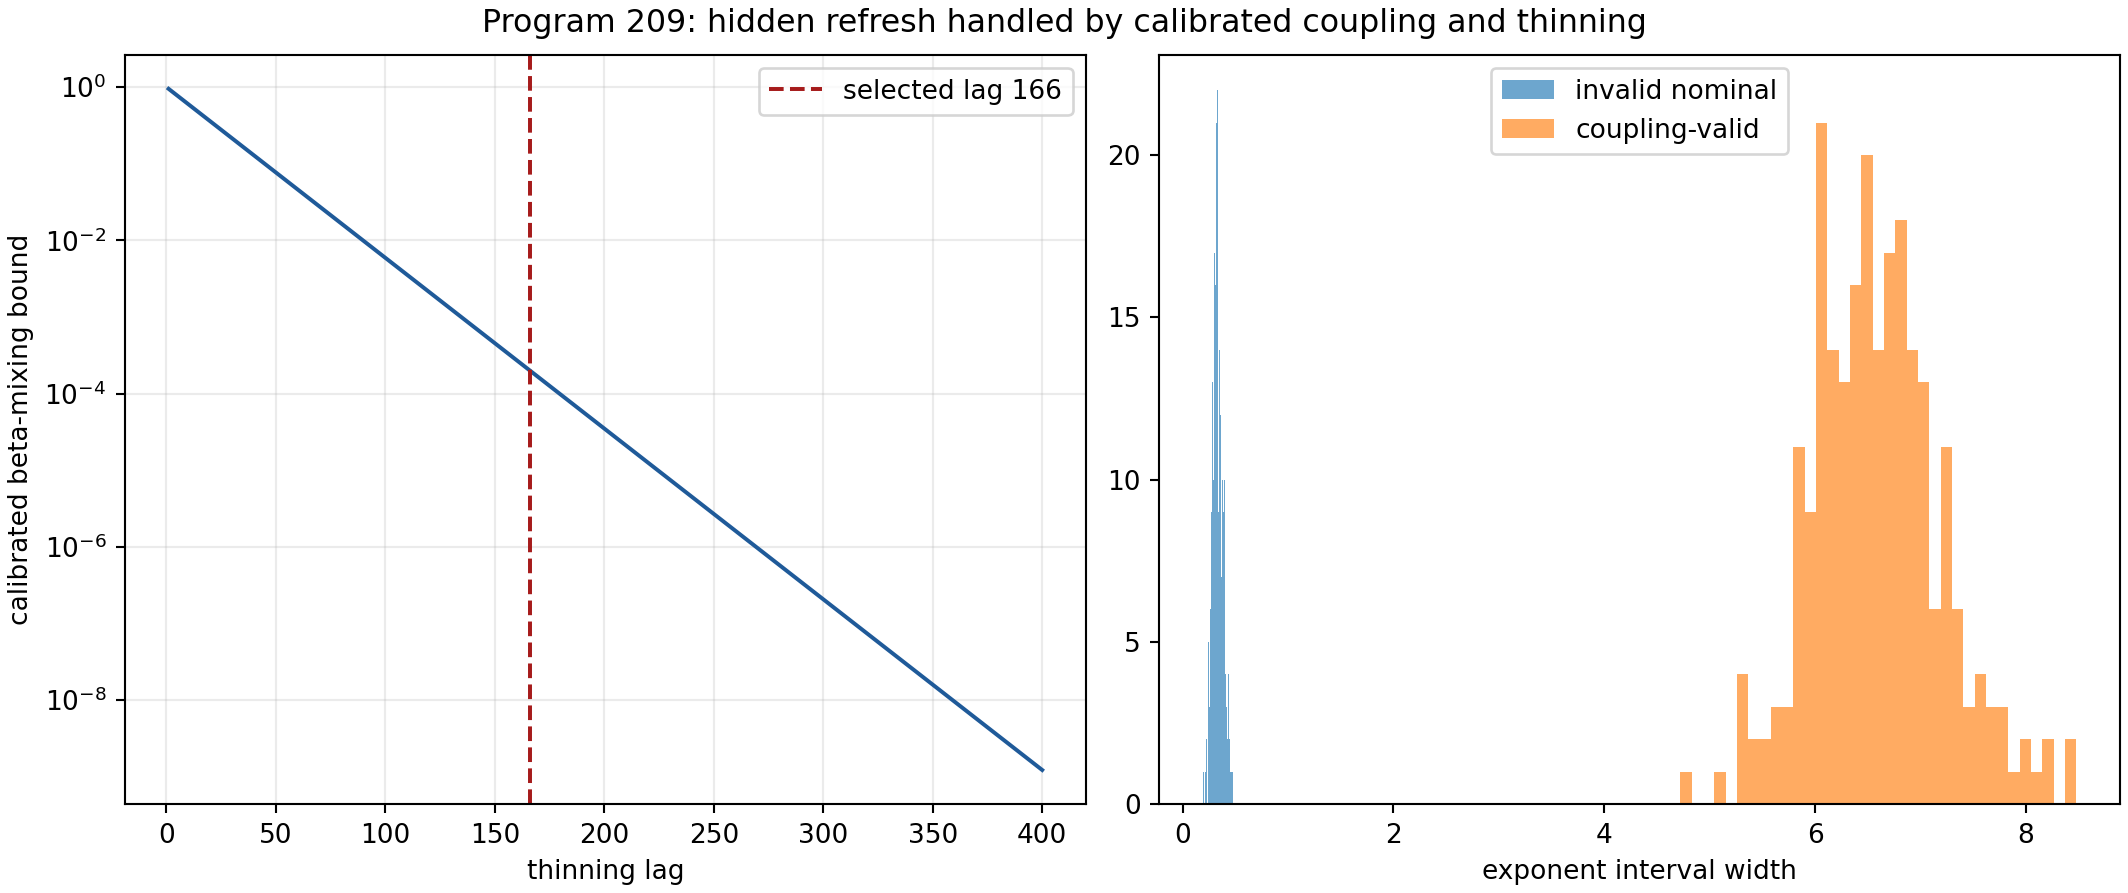
\includegraphics[width=0.94\textwidth]{FIN_Programs_204_216_Categorical_Catalytic_External_Figures/program209_hidden_mixing.png}
\caption{Calibrated thinning restores valid coverage under hidden geometric mixing at a substantial information cost.}
\end{figure}

\par\medskip\hrule\medskip

\chapter{Program 210 --- A time-uniform conformal e-process}

\section{Construction}

At sequential time \(t\), draw a fresh independent calibration block of \(m=15\) null records and one test record. Let

\[
r_t=
1+\#\{j:S_{tj}\ge S_t^{\rm test}\}.
\]

Under a continuous iid null, \(r_t\) is uniform on \(\{1,\ldots,m+1\}\). With

\[
H_{m+1}=\sum_{r=1}^{m+1}\frac1r,
\qquad
e_t=\frac{m+1}{H_{m+1}r_t},
\]

one has \(\mathbb E[e_t]=1\). Fresh independence makes

\[
E_T=\prod_{t=1}^Te_t
\]

a nonnegative martingale. Ville's inequality gives

\[
\Pr_0\left(\sup_TE_T\ge\frac1\alpha\right)\le\alpha.
\]

\section{Synthetic challenge}

At \(\alpha=0.05\), horizon \(20\), and 200 streams per model, the time-uniform rejection rates are:

\begin{center}
\begingroup\small
\setlength{\tabcolsep}{3.5pt}
\renewcommand{\arraystretch}{1.16}
\begin{longtable}{@{}p{0.331\textwidth}p{0.257\textwidth}p{0.271\textwidth}@{}}
\toprule
\textbf{Model} & \textbf{Rejection rate} & \textbf{Mean crossing time} \\
\midrule
\endhead
iid Gaussian & 0.02 & 9 among crossings \\
sorted & 1.00 & 2 \\
AR(1), coefficient 0.8 & 1.00 & 2 \\
repeated blocks & 1.00 & 2 \\
drift & 1.00 & 2 \\
\bottomrule
\end{longtable}
\endgroup
\end{center}

The exact null theorem is stronger than the simulation. The power figures are only synthetic evidence for the declared score.

\section{Limitation}

Fresh calibration makes the conditional expectation argument transparent but is experimentally expensive. Reusing one calibration set destroys the simple product-martingale proof and requires a new e-value construction.

\textbf{Verdict --- Proven null process; strong synthetic alternative power.}

\begin{figure}[htbp]
\centering
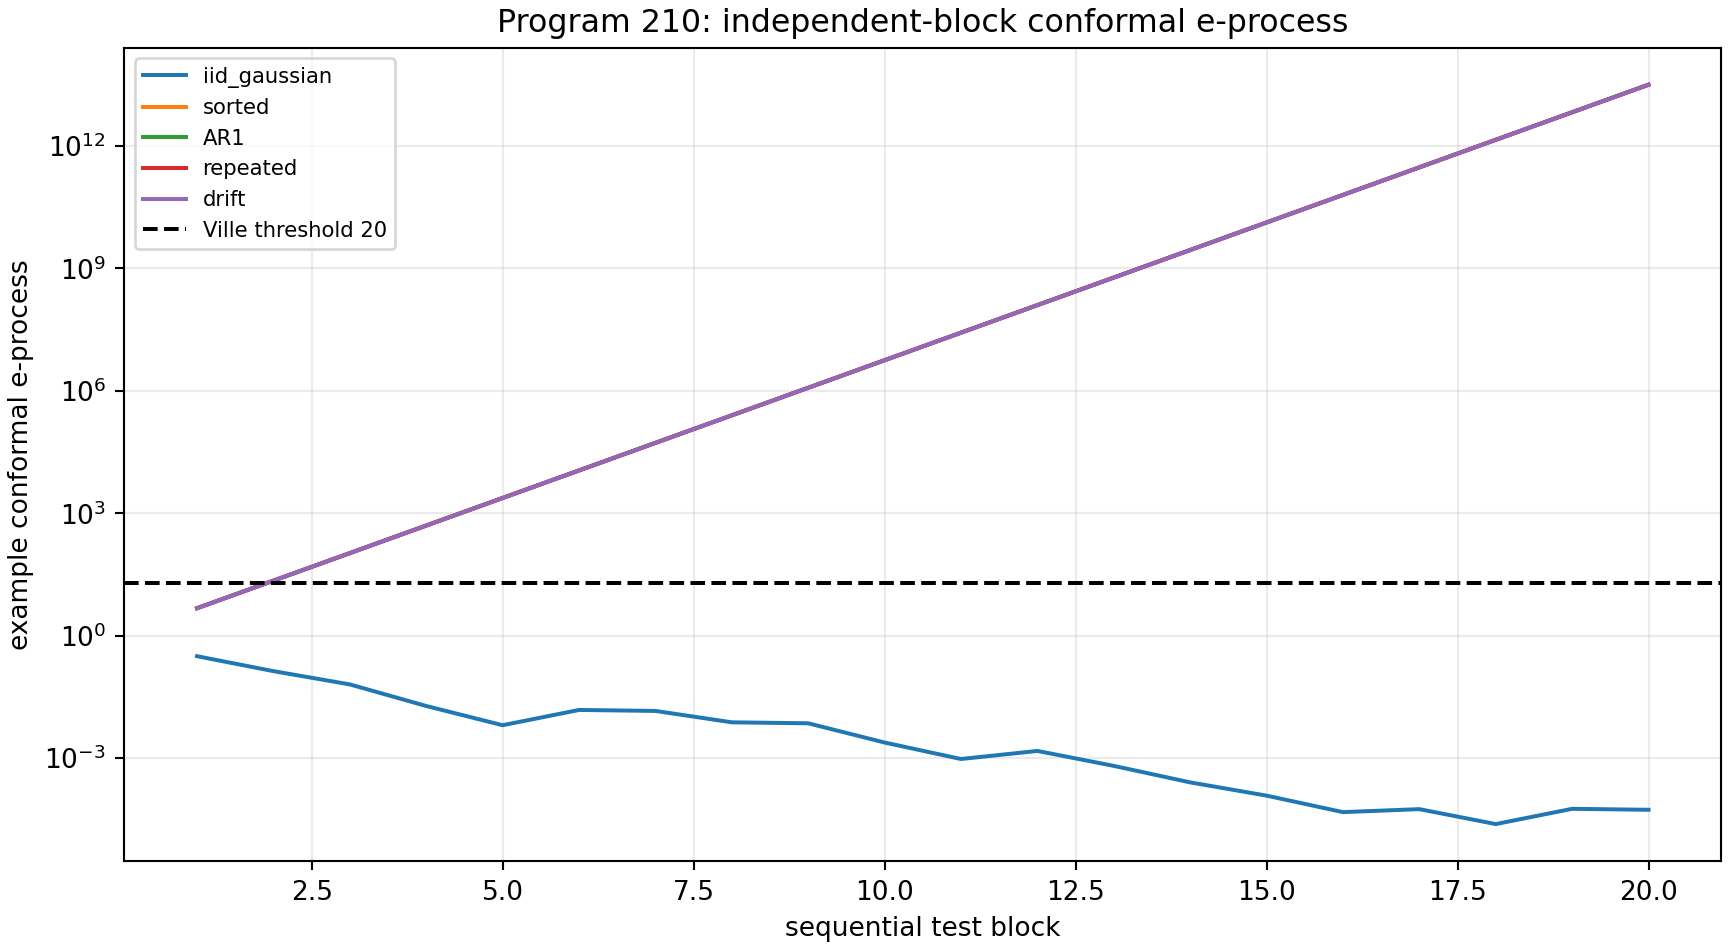
\includegraphics[width=0.94\textwidth]{FIN_Programs_204_216_Categorical_Catalytic_External_Figures/program210_conformal_eprocess.png}
\caption{A fresh-block conformal e-process maintains time-uniform null control and rapidly rejects the declared temporal alternatives.}
\end{figure}

\par\medskip\hrule\medskip

\chapter{Program 211 --- Finite-shot process tomography}

\section{Observation model}

The minimal Gaussian two-step frame uses single, plus, and echo contexts. Each context is measured at phases \(0\) and \(\pi\), producing six independent binomial counts. Their contrasts estimate three visibilities, which determine detector blur \(b\), increment variance \(v\), and temporal covariance \(c\) through a log-linear map.

\section{Simultaneous region}

Each count receives a two-sided Clopper--Pearson interval with Bonferroni allocation over the six observations. Monotone interval arithmetic transports these bounds through contrasts and logarithms. The result is intersected with

\[
0<b\le1,
\qquad
v\ge0,
\qquad
|c|\le v.
\]

Because each primitive interval has exact binomial coverage and the transport contains every compatible parameter value, the simultaneous region inherits the declared familywise guarantee.

\section{Simulation}

For truth

\[
(b,v,c)=(0.84,0.45,0.20),
\]

1000 shots per phase and context, and 600 repetitions:

\begin{itemize}
\item 
all 600 physical regions are nonempty;

\item 
simultaneous empirical coverage is \(1.0\);

\item 
memory-detection power is \(1.0\);

\item 
mean widths for \((\log b,v,c)\) are respectively \(0.652869\), \(0.928039\), and \(0.275170\).

\end{itemize}

The excess over nominal coverage is consistent with conservative Bonferroni and interval transport.

\textbf{Verdict --- Proven coverage construction within the Gaussian visibility model; strong finite-shot evidence.}

\begin{figure}[htbp]
\centering
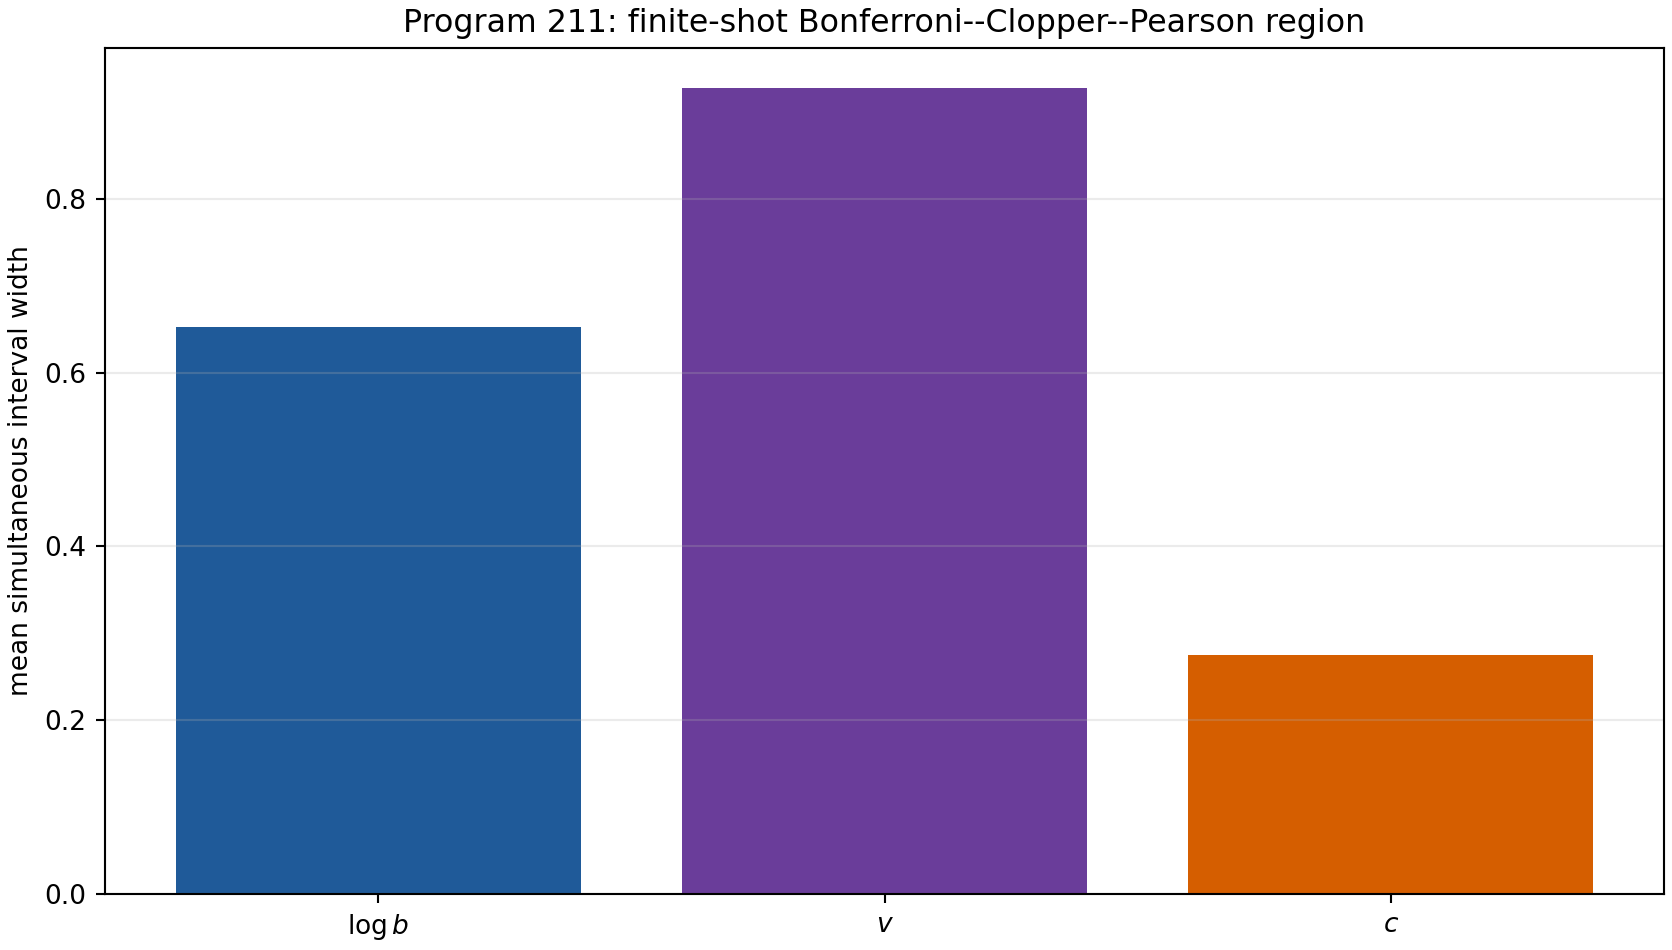
\includegraphics[width=0.94\textwidth]{FIN_Programs_204_216_Categorical_Catalytic_External_Figures/program211_finite_shot_tomography.png}
\caption{Finite-shot simultaneous regions cover the Gaussian process parameters and detect the declared memory term.}
\end{figure}

\par\medskip\hrule\medskip

\chapter{Program 212 --- Sharp environmental moment bounds}

Let \(\mu\) be a real symmetric probability measure on the circle and

\[
c_k=\int\cos(k\theta)\,d\mu(\theta).
\]

Positive definiteness requires the order-two Toeplitz matrix

\[
T_2=
\begin{pmatrix}
1&c_1&c_2\\
c_1&1&c_1\\
c_2&c_1&1
\end{pmatrix}
\]

to be positive semidefinite. Its determinant factors as

\[
\det T_2=(1-c_2)(1+c_2-2c_1^2).
\]

Together with the principal minors this yields

\[
2c_1^2-1\le c_2\le1.
\]

For \(c_1=4/5\),

\[
\frac7{25}\le c_2\le1.
\]

Both bounds are sharp.

\begin{itemize}
\item 
The lower bound is attained by equal atoms at \(\pm\arccos(4/5)\).

\item 
The upper bound is attained by mass \(9/10\) at \(0\) and \(1/10\) at \(\pi\).

\end{itemize}

The minimum numerical eigenvalue over a dense interval grid is \(-2.52\times10^{-16}\), consistent with roundoff at the semidefinite boundary.

This theorem bounds an unmeasured two-time visibility from a measured one-time visibility. It does not select a microscopic environment within the interval.

\textbf{Verdict --- Proven and sharp.}

\begin{figure}[htbp]
\centering
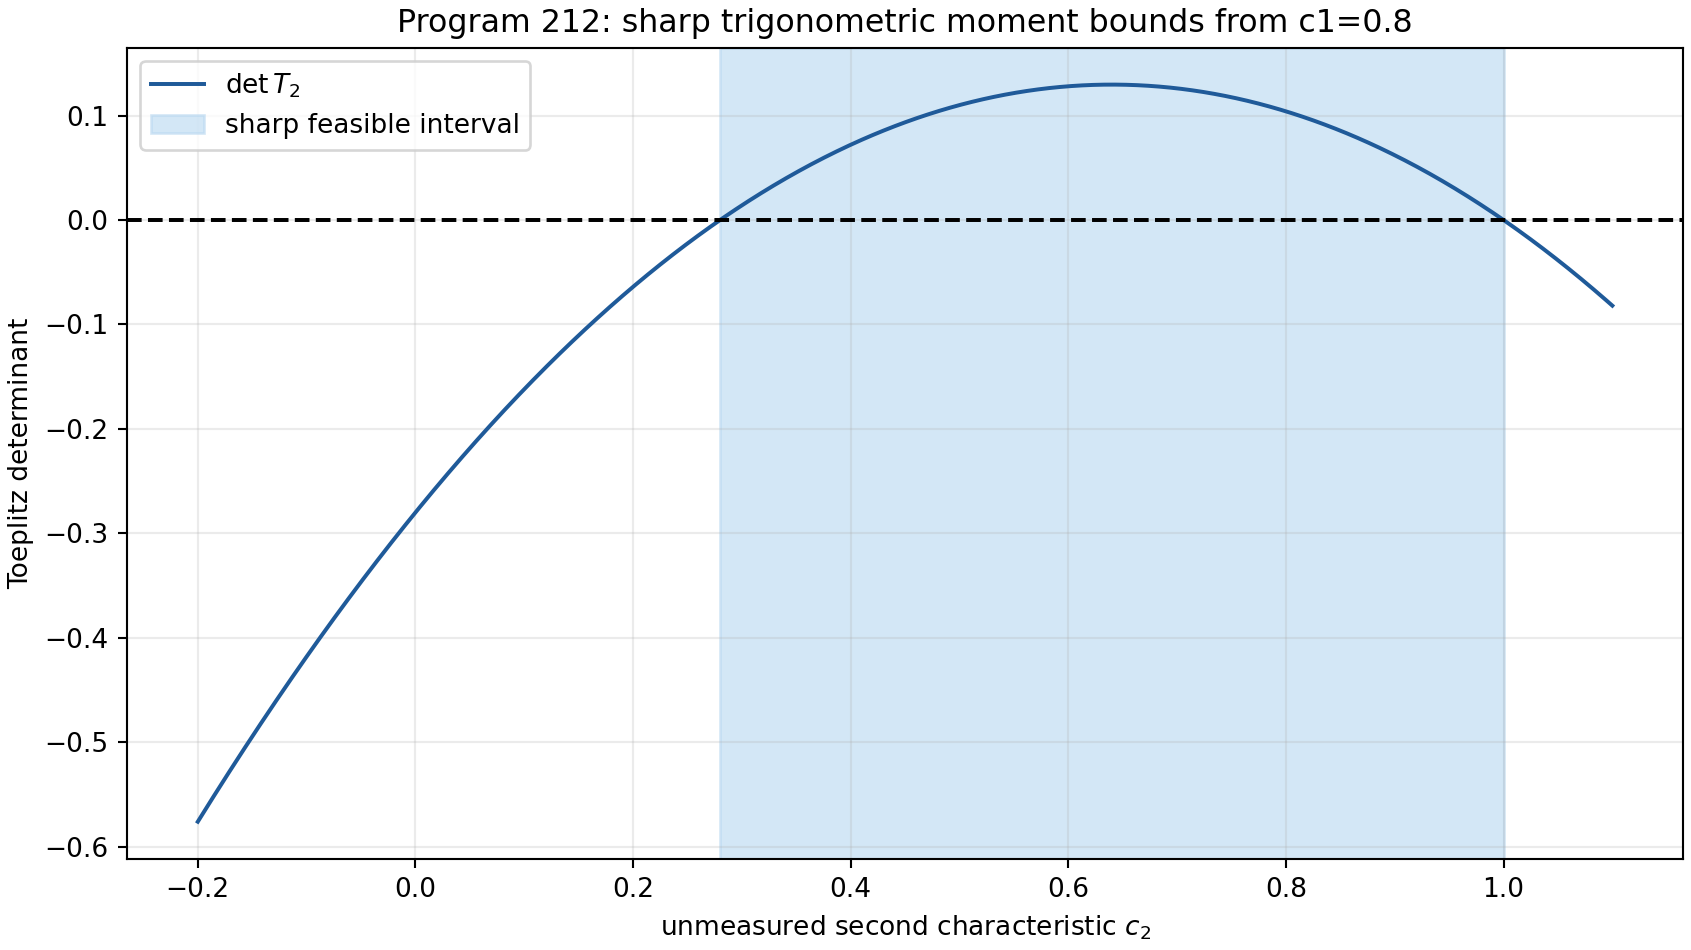
\includegraphics[width=0.94\textwidth]{FIN_Programs_204_216_Categorical_Catalytic_External_Figures/program212_environment_moments.png}
\caption{Toeplitz positivity gives the sharp environmental moment interval \(7/25\le c_2\le1\).}
\end{figure}

\par\medskip\hrule\medskip

\chapter{Program 213 --- Phase naturality hierarchy}

\section{Continuous homomorphisms}

Every continuous group homomorphism

\[
h:U(1)\longrightarrow U(1)
\]

has the form \(h(z)=z^n\) for some integer \(n\). Program 213 studies the oscillatory step datum

\[
z_\ell=e^{i\omega_\ell}=e^{i\pi/4},
\]

which has order eight. This is distinct from the legacy offset \(\phi_\ell=\pi/6\). Natural endomorphisms keep the order-eight datum torsion.

The strict target \(e^{i\,743/4000}\) is non-torsion: equality to a root of unity would imply a rational identity for \(\pi\).

\section{Measurable and cocycle extensions}

Borel measurable homomorphisms between locally compact second-countable groups are automatically continuous. They therefore reduce to the same integer-degree family.

For a trivial group action, a normalized continuous one-cocycle satisfies

\[
c(gh)=c(g)c(h),
\]

which is again the homomorphism equation. This larger vocabulary does not enlarge the image class.

Unrestricted holomorphic interpolation can hit the strict phase at a chosen point, but only by inserting a coefficient that depends on the target. Such a map is not a target-independent source theorem.

\textbf{Verdict --- Proven in the declared naturality hierarchy.} No origin, orientation, or strict phase source is exported.

\begin{figure}[htbp]
\centering
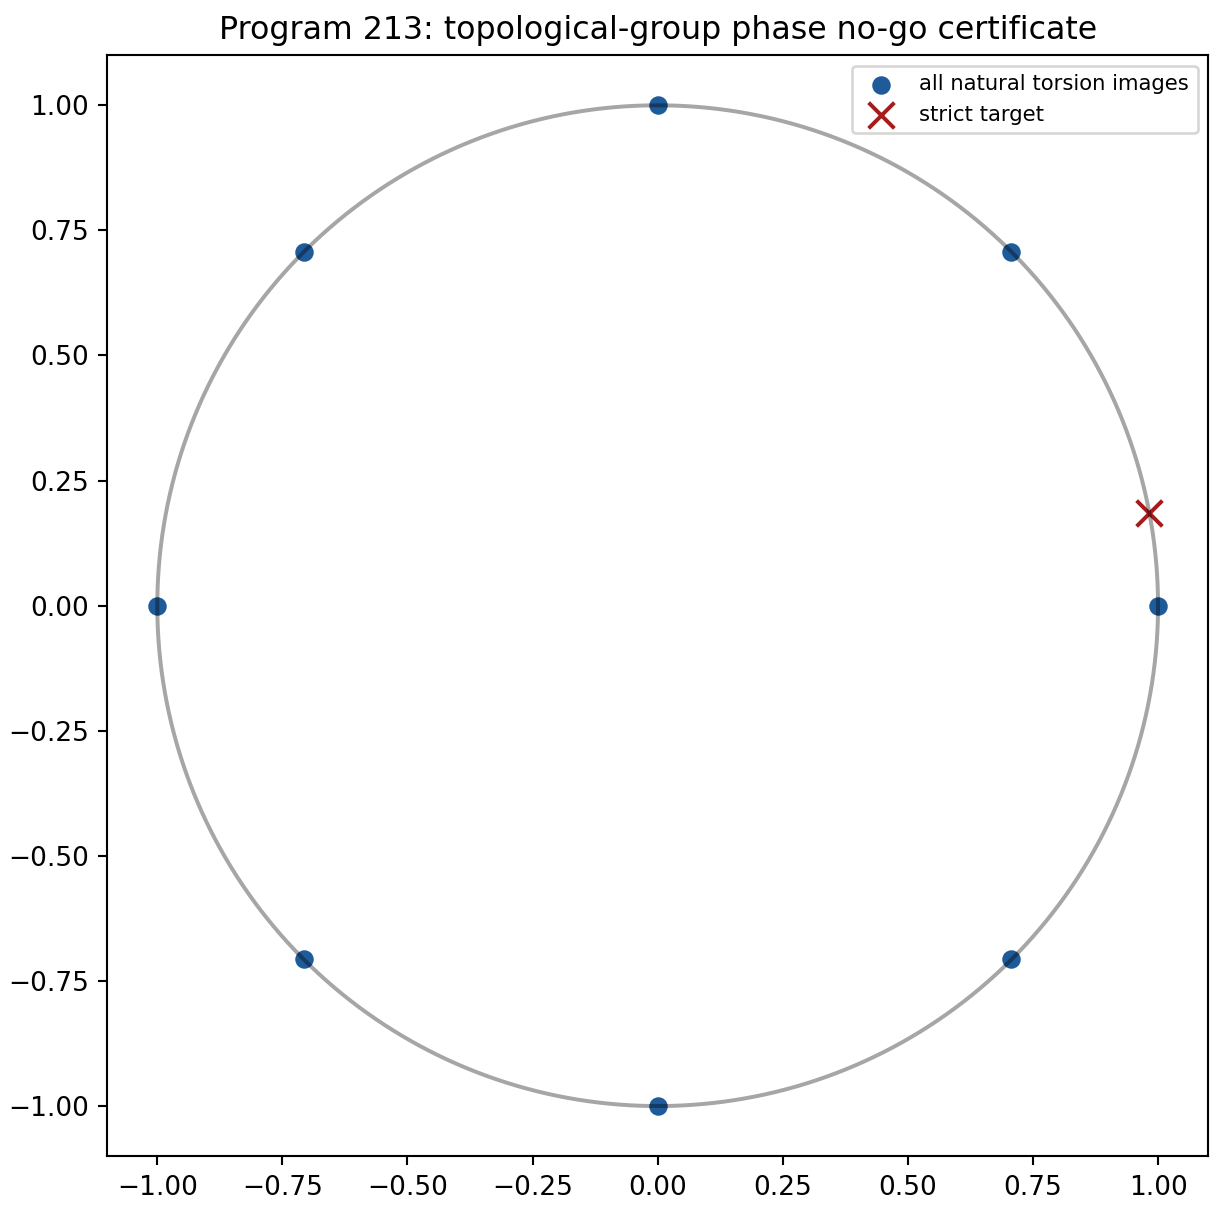
\includegraphics[width=0.94\textwidth]{FIN_Programs_204_216_Categorical_Catalytic_External_Figures/program213_phase_no_go.png}
\caption{Natural endomorphisms keep the legacy oscillatory datum in its finite torsion orbit and miss the strict non-torsion target.}
\end{figure}

\par\medskip\hrule\medskip

\chapter{Program 214 --- Scale-free spectral fingerprint}

\section{Frozen protocol}

Let the eigenvalues of the twelve-node strict generator be

\[
0=\lambda_0<\lambda_1\le\cdots\le\lambda_{11}.
\]

The projective fingerprint is

\[
\Sigma(A)=
\left(
\frac{\lambda_1}{\lambda_{11}},
\ldots,
\frac{\lambda_{10}}{\lambda_{11}},
1
\right),
\]

provided \(A\) is positive semidefinite with exactly one zero eigenvalue. Acceptance requires

\[
\|\Sigma(A_{\rm candidate})-\Sigma(A_{\rm strict})\|_\infty\le0.02.
\]

The protocol, threshold, structural gate, and target signature are frozen in a preregistration file before external execution.

\section{Internal challenges}

The exact target signature begins

\[
(0.3219737582,0.3219737582,
0.6733249110,0.6733249110,\ldots,1).
\]

Six scale factors from \(10^{-6}\) to \(10^6\) pass with distances below \(1.3\times10^{-15}\). A random node permutation also passes. One-percent symmetric edge noise passes with distance \(0.00233262\).

Three alternatives fail:

\begin{itemize}
\item 
ten-percent edge noise: distance \(0.0420993\);

\item 
nearest-neighbour cycle: distance \(0.423325\);

\item 
raw legacy generator: structural PSD failure with minimum eigenvalue \(-21.3771\).

\end{itemize}

The legacy failure is not a global rejection of the legacy bridge object. It says only that the raw legacy matrix is not an admissible instance of this strict positive-generator fingerprint.

\section{Physical boundary}

Projective normalization removes an overall operator scale. That is useful before a physical clock exists. It also means the protocol cannot determine energy or time units. An apparatus must first reconstruct an operator or its spectrum from independent data.

\textbf{Verdict --- Proven invariance and computer-assisted finite falsification.} The protocol is ready for, but has not undergone, external empirical testing.

\begin{figure}[htbp]
\centering
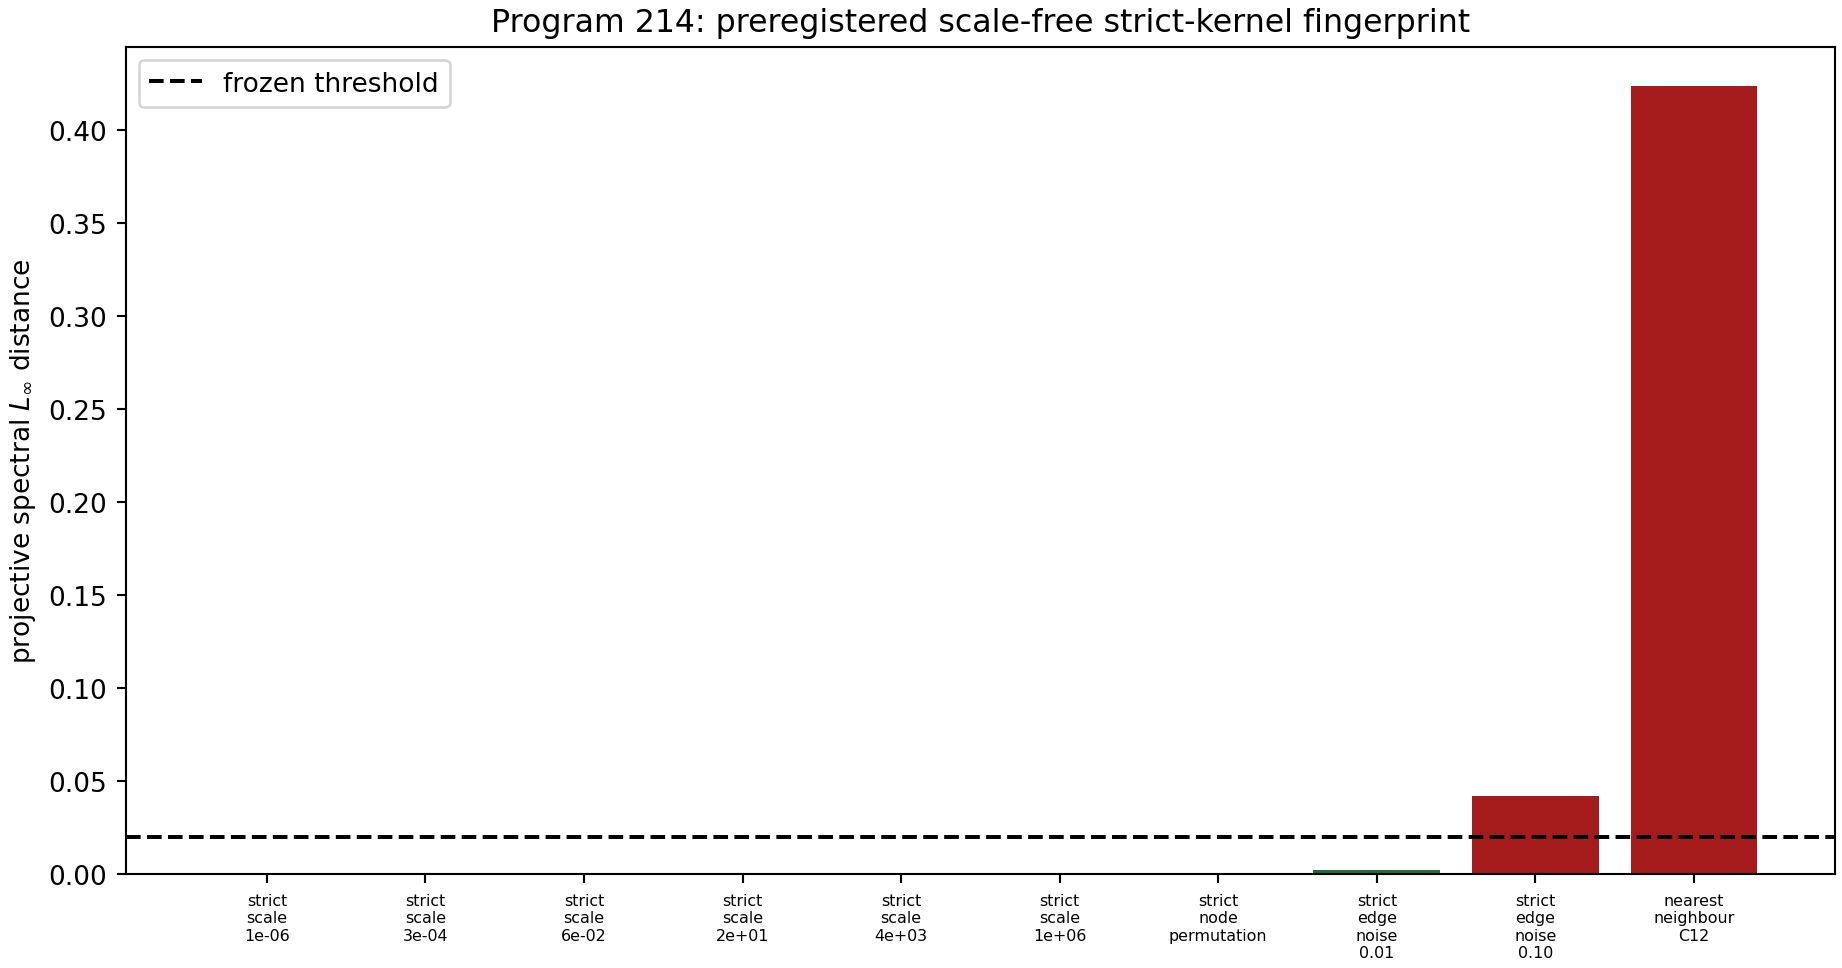
\includegraphics[width=0.94\textwidth]{FIN_Programs_204_216_Categorical_Catalytic_External_Figures/program214_scale_free_protocol.png}
\caption{The frozen projective fingerprint accepts exact rescalings and small perturbation, while rejecting large and structurally incompatible alternatives.}
\end{figure}

\par\medskip\hrule\medskip

\chapter{Program 215 --- Independent external-data gate}

The eleven required fields cover provenance, ordered raw events, preparation, intervention, clock, detector calibration, environmental record, frozen analysis, negative controls, held-out target, and an independent-analysis boundary.

Three local external-lineage candidates pass respectively \(1/11\), \(2/11\), and \(1/11\) fields. The earlier synthetic operational bundle passes \(10/11\) but fails independent provenance. It is correctly classified as method validation.

No web search or Firecrawl was used. No local candidate is admitted. A machine-readable request contract states exactly what a future provider must supply.

\textbf{Verdict --- Proven for the current local intake scope.} No external physical record exists in the admitted analysis set.

\begin{figure}[htbp]
\centering
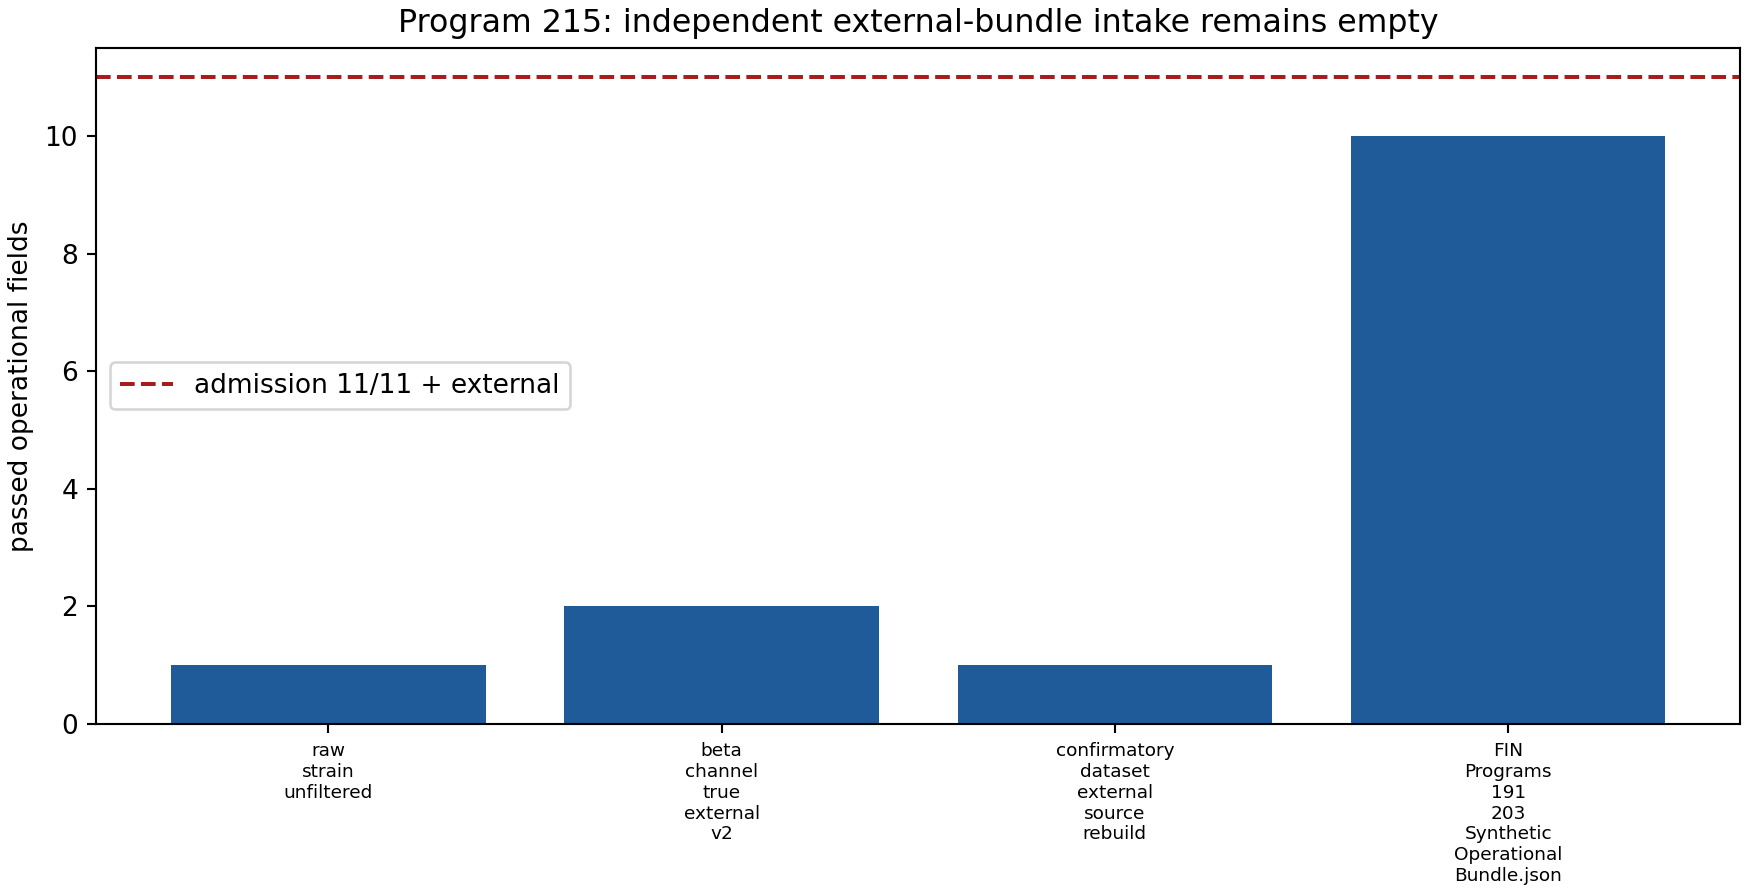
\includegraphics[width=0.94\textwidth]{FIN_Programs_204_216_Categorical_Catalytic_External_Figures/program215_external_bundle.png}
\caption{No local candidate satisfies the independent eleven-field external intake gate.}
\end{figure}

\par\medskip\hrule\medskip

\chapter{Program 216 --- Conditional prediction lock}

The external prediction file freezes:

\begin{itemize}
\item 
the input schema;

\item 
the Program-215 admission dependency;

\item 
the spectral reconstruction and projective fingerprint;

\item 
the held-out quantity;

\item 
the decision threshold;

\item 
negative controls;

\item 
failure and reporting rules.

\end{itemize}

Its execution condition is boolean and explicit:

\[
\text{execute Program 216}
\iff
\text{Program 215 admits an independent 11/11 bundle}.
\]

Because the antecedent is false, no external prediction is computed. The earlier synthetic dry run is not recycled as physical evidence.

\textbf{Verdict --- Proven gate status.} The prediction protocol exists; experimental validation does not.

\begin{figure}[htbp]
\centering
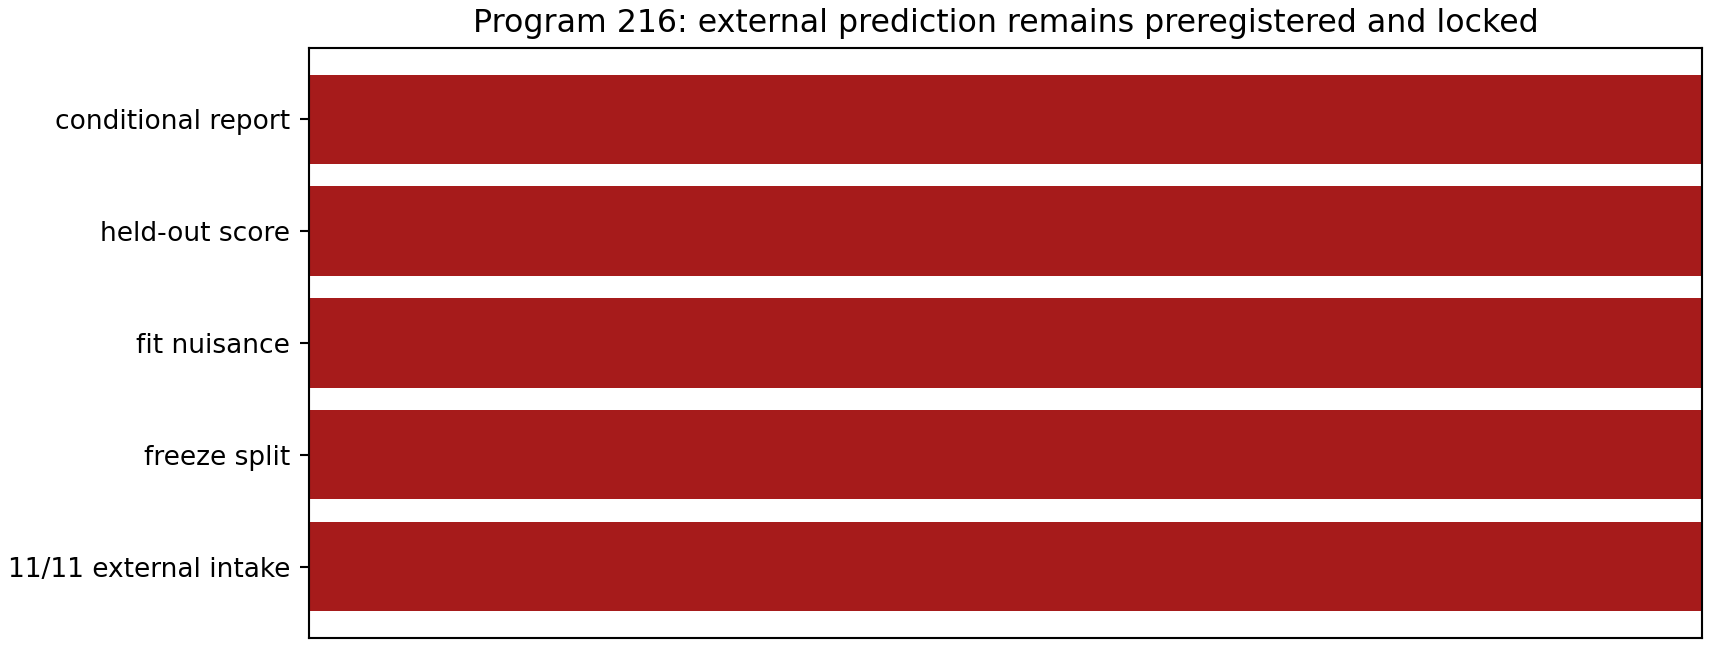
\includegraphics[width=0.94\textwidth]{FIN_Programs_204_216_Categorical_Catalytic_External_Figures/program216_external_prediction_lock.png}
\caption{The external prediction remains locked because the prerequisite independent bundle is absent.}
\end{figure}

\par\medskip\hrule\medskip

\chapter{Cross-program synthesis}

\section{The new object stack}

The results support the following dependency diagram:

\[
\boxed{A}
\longrightarrow
\begin{cases}
e^{-itA}\\
e^{-tA}\\
(A+zI)^{-1}
\end{cases}
\]

but

\[
A
\not\Longrightarrow
\rho,\;
\text{orientation reference},\;
\text{physical unit},\;
\text{instrument},\;
\text{external record}.
\]

Program 204 proves that a central state is extra unless a morphism principle is added. Program 208 proves that an orientation reference is both sufficient and resource-bearing. Programs 209--212 construct statistically and operationally meaningful inference only after an acquisition class and apparatus model are declared. Programs 214--216 prove that even a strong scale-free internal fingerprint remains prephysical until an independent record passes intake.

\section{Observer paradox}

The same \(A\) generates reversible wave dynamics and irreversible-looking diffusion:

\[
U_t=e^{-itA},
\qquad
P_t=e^{-tA}.
\]

This does not create a contradiction. The two maps solve different evolution equations and use different time structures. An operational observer sees a record only after preparation, coupling to an environment, coarse graining, and measurement.

The perfect reference theorem adds a sharper statement. An observer capable of distinguishing a direction may carry an asymmetric reference state. That reference can be reused to orient operations, but its existence is not explained by an orientation-blind generator. The "observer paradox" is therefore not resolved by choosing wave over diffusion. It is typed as the provenance problem for the state, clock, reference frame, environment, instrument, and record.

\section{Information loss}

\(P_t\) contracts nonconstant spectral modes:

\[
\|P_tf-\Pi_0f\|_2
\le
e^{-t\lambda_1}\|f-\Pi_0f\|_2.
\]

This is mathematical coarse graining. Calling it physical information loss requires a probability state, an operational distinction measure, a clock, and an environment or discarded subsystem. Program 212 shows that even one measured dephasing moment leaves a sharp interval of compatible two-time environments. No unique microscopic loss mechanism follows from the reduced semigroup alone.

\section{The status of a Lagrangian}

For a positive generator \(A=L+m^2I\) and source \(J\), the quadratic action

\[
S[\phi]
=
\frac12\phi^\mathsf TA\phi-J^\mathsf T\phi
\]

has stationary equation

\[
A\phi=J,
\qquad
\phi=A^{-1}J.
\]

Thus reconstruction of a minimal quadratic action from a Green operator is mathematically legitimate. Adding an operator potential,

\[
S[\phi,K]
=
\frac12\phi^\mathsf T(L+m^2I)\phi-J^\mathsf T\phi
+
\operatorname{tr}V(K)-\operatorname{tr}(KC),
\]

requires a separately specified variation domain and source \(C\). Nothing in Programs 204--216 supplies the missing tensor-resolved Lagrangian source or reverses the existing obstruction results. The action remains a conditional representation, not a physical closure.

\section{Deepest surviving interpretation}

The deepest interpretation that survives this round is:

\begin{quote}\itshape
FIN is a dimensionless spectral-information generator equipped with a developing operational completion problem. Its self-adjoint operator unifies wave, diffusion, and Green dynamics. States, symmetry-breaking references, scale sections, interventions, instruments, environments, and independent records are additional typed objects. Some can be classified or bounded; none is presently forced in the unique physical form required for experimental theory.

\end{quote}

This conclusion is stronger than saying merely that "more physics is needed." It identifies which data are absent and proves several impossibility and sufficiency theorems about them.

\par\medskip\hrule\medskip

\chapter{Falsification ledger}

\section{Claims that survived}

\begin{itemize}
\item 
Uniform central weighting is unique under the explicit Morita-permutation premise.

\item 
All-unital-homomorphism state naturality is inconsistent with automorphism-uniform states.

\item 
Continuous exponent cocycles are linear and do not select \(9/5\).

\item 
Invariant catalysts cannot repair the declared reflection-conversion inequality.

\item 
A perfect asymmetric reference enables exact arbitrary-target conversion.

\item 
Berbee coupling plus DKW gives a valid hidden-mixing bound under a calibrated envelope.

\item 
The independent-block conformal product is an e-process.

\item 
The finite-shot region has the declared simultaneous coverage guarantee.

\item 
The order-two moment interval is sharp.

\item 
The stated phase naturality hierarchy cannot generate the strict phase.

\item 
The projective spectral fingerprint is exactly scale invariant.

\end{itemize}

\section{Claims deliberately rejected or left open}

\begin{itemize}
\item 
"Morita theory automatically chooses \(9/5\)": rejected without the extra permutation/\allowbreak{}state premise.

\item 
"A semigroup determines the strict exponent": rejected.

\item 
"A contract is a formal certificate": rejected.

\item 
"The entire Lean library is verified": rejected.

\item 
"Catalysis solves the strict selector": rejected; the catalyst supplies it.

\item 
"Nominal iid uncertainty remains valid under hidden refresh": falsified in the challenge.

\item 
"A one-time channel identifies its environment": rejected by the sharp moment interval and previous counterexamples.

\item 
"Projective operator agreement supplies physical units": rejected.

\item 
"A synthetic 10/\allowbreak{}11 bundle is external evidence": rejected.

\item 
"A frozen prediction counts as validation": rejected.

\end{itemize}

\section{Robustness boundary}

Every positive conclusion is conditional on its declared class:

\begin{itemize}
\item 
change the morphism category, and the central-state theorem changes;

\item 
drop continuity, and pathological additive cocycles exist;

\item 
allow a symmetry-bearing catalyst, and the invariant no-help theorem no longer applies;

\item 
remove the mixing-rate calibration, and Program 209 has no finite guarantee;

\item 
reuse calibration records, and Program 210 needs a new proof;

\item 
leave the Gaussian visibility family, and Program 211 needs a new likelihood;

\item 
increase the moment order, and Program 212 becomes a larger semidefinite problem;

\item 
abandon naturality, and target-coded phase interpolation is trivial;

\item 
change the finite graph or reconstruction map, and Program 214 tests a different object.

\end{itemize}

This scoped form is a strength: each theorem has a visible falsification surface.

\par\medskip\hrule\medskip

\chapter{Recommended Programs 217--229}

The next round should not repeat closed selector, bridge, or Lagrangian lanes. It should attack the new obligations created by Programs 204--216.

\section{Program 217 --- Provenance of the Morita-permutation axiom}

\textbf{Question:} Can a preparation or coarse-graining principle derive uniform central weights without inserting them?

Construct a category whose objects are finite semisimple observable algebras with specified operational embeddings and whose morphisms preserve preparation statistics. Classify natural states on that restricted category. The decisive output is either a uniqueness theorem with a physically interpretable morphism class or a proof that a central measure remains free.

\textbf{Priority:} very high.\\
\textbf{Probability of useful theorem:} \(0.75\).\\
\textbf{Closure boundary:} do not call a categorical symmetry a physical preparation until an instrument realizes it.

\section{Program 218 --- Target-independent exponent generator}

\textbf{Question:} Can \(\eta=9/5\) be a stable eigenvalue of a flow whose generator is defined without the target?

Search polynomial and variational beta functions

\[
\dot\eta=F(\eta;\mathcal D)
\]

where \(\mathcal D\) is strict-derived data and contains no occurrence of \(9/5\). Require structural stability, basin information, and independence from the fitting interval. If no admissible \(F\) exists in a declared finite class, publish a no-go certificate.

\textbf{Priority:} high.\\
\textbf{Probability of strict source:} \(0.15\); probability of a useful no-go: \(0.70\).

\section{Program 219 --- Execute the pinned Arb certificate}

Build the exact environment specified by Program 206, record all dependency hashes, and run the common directed-rounding computation. The acceptance criterion must remain frozen at a worst enclosure below \(0.03\).

\textbf{Priority:} high infrastructure.\\
\textbf{Probability of completion with authorized dependencies:} \(0.80\).\\
\textbf{Failure is informative:} a bound above threshold must be reported as a failed certificate.

\section{Program 220 --- Complete the Mathlib Lean build}

Pin Lean and Mathlib commits, generate lake-manifest.json, compile the general source, and repair type or API errors without weakening statements. Then add semigroup theorems or explicitly separate what remains analytic.

\textbf{Priority:} high infrastructure.\\
\textbf{Probability of core Dirichlet closure:} \(0.85\).\\
\textbf{Probability of entrywise heat positivity in the first pass:} \(0.55\).

\section{Program 221 --- Cost and degradation of finite symmetry references}

The perfect catalyst of Program 208 is reusable because its orbit states are orthogonal. Quantify approximate conversion when the reference states are not orthogonal. Derive a trade-off among conversion error, reference disturbance, orbit distinguishability, and number of uses.

\textbf{Priority:} very high theoretical.\\
\textbf{Probability of a quantitative theorem:} \(0.70\).\\
\textbf{Relevance:} this converts the binary selector obstruction into a finite resource budget without pretending to source the budget.

\section{Program 222 --- Optimal hidden-mixing acquisition design}

Minimize the width of the Program-209 confidence interval over lag, record length, and allocation of the coupling/\allowbreak{}DKW failure budget. Compare thinning with blocking and median-of-means constructions.

\textbf{Priority:} medium-high.\\
\textbf{Probability of useful method improvement:} \(0.85\).\\
\textbf{Required report:} valid coverage, effective sample size, and information cost on the same challenge family.

\section{Program 223 --- Reusable-calibration sequential e-process}

Construct an anytime-valid conformal or betting process that can reuse a finite calibration set without assuming independent fresh blocks at every time. Candidate tools are conditional randomization, leave-one-out ranks, and test martingales with predictable betting functions.

\textbf{Priority:} high operational.\\
\textbf{Probability of a scoped theorem:} \(0.60\).\\
\textbf{Falsification:} demonstrate whether naive calibration reuse violates Ville control.

\section{Program 224 --- Near-optimal finite-shot tomography regions}

Replace the conservative Bonferroni transport by inversion of the joint binomial likelihood or an exact likelihood-ratio region. Prove or conservatively certify coverage, then compare volume and memory-detection power with Program 211.

\textbf{Priority:} medium-high.\\
\textbf{Probability of substantial width reduction:} \(0.80\).

\section{Program 225 --- Higher environmental moment hierarchy}

Extend Program 212 from \(T_2\) to \(T_n\). Compute semidefinite bounds on unmeasured \(c_k\), extract extremal atomic measures, and determine the minimum number of time contrasts needed to distinguish declared environment classes.

\textbf{Priority:} very high.\\
\textbf{Probability of exact low-order results:} \(0.90\).\\
\textbf{Physical boundary:} moment reconstruction remains an operational environment quotient unless microscopic access is supplied.

\section{Program 226 --- Phase obstruction with nontrivial actions}

Study continuous and measurable one-cocycles for nontrivial \(U(1)\) or finite cyclic actions, together with equivariant cohomology and central extensions. Demand a target-independent source law and an origin/\allowbreak{}orientation theorem.

\textbf{Priority:} medium.\\
\textbf{Probability of strict phase source:} \(0.10\); probability of a stronger no-go theorem: \(0.65\).

\section{Program 227 --- Spectral reconstruction from an explicit instrument}

Construct a complete observation map from preparations and time-stamped measurements to estimates of the nonzero eigenvalue ratios of \(A\). Prove identifiability modulo scale and node relabeling, and propagate finite-shot uncertainty into the Program-214 fingerprint distance.

\textbf{Priority:} highest physics-bridge task.\\
\textbf{Probability of a finite-model theorem:} \(0.75\).

\section{Program 228 --- Acquire one independent 11/\allowbreak{}11 bundle}

Use the Program-215 request contract to obtain a genuinely independent, ordered, raw experimental record with apparatus calibration, negative controls, and a held-out target. Do not alter the intake criteria after viewing the data.

\textbf{Priority:} highest empirical task.\\
\textbf{Probability cannot be estimated mathematically:} it depends on external coordination and apparatus access.

\section{Program 229 --- Execute the locked external prediction}

Only if Program 228 passes all eleven fields, hash the admitted bundle, execute the frozen Program-216 pipeline once, report the primary result and all negative controls, and retain failure without model repair.

\textbf{Priority:} conditional on Program 228.\\
\textbf{Scientific value:} decisive for distinguishing an internally coherent operator model from an experimentally supported physical model.

\section{Ranked roadmap}

\begin{center}
\begingroup\small
\setlength{\tabcolsep}{3.5pt}
\renewcommand{\arraystretch}{1.16}
\begin{longtable}{@{}p{0.160\textwidth}p{0.280\textwidth}p{0.420\textwidth}@{}}
\toprule
\textbf{Rank} & \textbf{Program} & \textbf{Reason} \\
\midrule
\endhead
1 & 227 & supplies the missing mathematical map from apparatus records to the spectral fingerprint \\
2 & 228 & supplies the missing independent empirical object \\
3 & 221 & quantifies the selector as a resource instead of replaying a symmetry no-go \\
4 & 225 & extends a sharp theorem into testable temporal constraints \\
5 & 220 & closes formal proof debt with an available local Lean toolchain \\
6 & 219 & closes the remaining numerical-certificate debt \\
7 & 217 & determines whether \(9/5\) has categorical or merely stipulated status \\
8 & 223 & makes sequential falsification operationally economical \\
9 & 224 & reduces tomography conservatism \\
10 & 222 & improves hidden-dependence efficiency \\
11 & 218 & high conceptual value but low strict-source probability \\
12 & 226 & likely to strengthen a no-go rather than source the phase \\
13 & 229 & decisive, but admissible only after Program 228 \\
\bottomrule
\end{longtable}
\endgroup
\end{center}

\par\medskip\hrule\medskip

\chapter{Final answer}

Programs 204--216 do not discover a theorem that forces FIN to become physics. They discover something more precise.

The spectral generator is sufficient for a common mathematical dynamics. Morita-permutation symmetry can conditionally select a central measure. A perfect asymmetric reference can operationally supply a selector. Mixing assumptions and finite-shot instruments can support rigorous inference. Toeplitz positivity can turn one environmental moment into sharp bounds on another. Projective spectral data can support a scale-free falsification protocol.

None of these constructions eliminates its premise. Uniform central measure, perfect orientation reference, mixing calibration, apparatus model, and independent record remain typed inputs unless a new theorem or experiment supplies them.

The deepest surviving result is therefore:

\begin{quote}\itshape
The missing bridge is not one scalar constant and not another kernel. It is an operational section of the spectral theory: a compatible choice of state, symmetry reference, scale and clock, intervention, instrument, environment class, and independent record. Programs 204--216 prove exact uniqueness, sufficiency, no-go, and uncertainty statements for parts of this section, while proving that the complete section is not yet forced by the strict operator.

\end{quote}

This is the correct point from which Programs 217--229 should proceed.

\par\medskip\hrule\medskip

\chapter{Reproducibility}

Run:

python3 fin\_programs\_204\_216\_categorical\_catalytic\_external.py python3 -m unittest -v \\
test\_fin\_programs\_204\_216\_categorical\_catalytic\_external.py

The suite executes thirteen programs and 77 tests. Machine-readable outputs include the main result file, formal-environment contracts, the phase no-go certificate, the scale-free preregistration, the external bundle request, and the locked prediction protocol. The release manifest records cryptographic hashes after the final PDF is built.

Suggested citation:

\.Zuchowski, K. (2026). \emph{FIN Programs 204--216: Categorical Measures, Perfect References, and External Falsification Gates} (FIN Research Monograph, Release 10.19; Version 1.0.0) [Preprint]. Zenodo.


\clearpage
\chapter*{Release reproducibility}
\addcontentsline{toc}{chapter}{Release reproducibility}
\begin{Verbatim}[fontsize=\small]
python3 fin_programs_204_216_categorical_catalytic_external.py
python3 -m unittest -v \
  test_fin_programs_204_216_categorical_catalytic_external.py
\end{Verbatim}

Machine-readable results are stored in
\path{FIN_Programs_204_216_Categorical_Catalytic_External_Results.json}.
The release contains six frozen auxiliary contracts or certificates, two Lean
sources, 77 tests, and thirteen figures. The dependency-free Lean core probe
compiles locally; the Mathlib-dependent general graph library does not.

\medskip
\noindent\textbf{Suggested citation:}

\.Zuchowski, K. (2026). \emph{FIN Programs 204--216: Categorical Measures,
Perfect References, and External Falsification Gates}
(FIN Research Monograph, Release 10.19; Version 1.0.0) [Preprint]. Zenodo.
\end{document}
